\chapter{Experiments\label{cha:chapter4}}
\hspace*{1em}This chapter details the experiments conducted in the context of this thesis.
We evaluate the proposed methods on three image classification datasets:
MNIST \cite{lecun2010mnist},
CIFAR-10 \cite{krizhevsky2009learning},
and Imagenette \cite{DBLP:journals/information/HowardG20}, which is a subset of 10 easily classified classes from the ImageNet dataset.
First, we provide an overview of the experimental setup.
We then present the results of the gradient ratio thresholding method, as detailed in \cref{sec:nestedquantizationlayer},
followed by the results of the custom loss terms discussed in \cref{sec:customloss}.

% ------------------------------------------------------------
% ----------------------- Setup ----------------------- 
% ------------------------------------------------------------

\section{Experimental Setup}
\label{sec:setup}
\hspace*{1em}\textbf{Software and Hardware Setup.} As briefly mentioned in \cref{sec:nestedquantizationlayer},
our custom methods are implemented in TensorFlow.
Specifically, we used TensorFlow version 2.11.0, running on Python 3.10.14. 
All experiments are conducted on a server equipped with two NVIDIA A40 GPUs, 
each with 48 GB of memory, running on CUDA 11.4 and driver version 470.256.02.

\textbf{Experiment Networks.} 
For simplicity and tractability, we define custom networks for each dataset.
For MNIST, we use a small network consisting of two dense layers, 
each adjusted to incorporate nested quantization layers for both weights and biases. 
For CIFAR-10, we use a convolutional network with three blocks of convolutional layers, 
each adjusted to incorporate nested quantization layers for both kernels and biases.
These are followed by two dense layers.
The Imagenette model is a ResNet-inspired architecture,
featuring an initial quantized convolutional block followed by four stages of residual blocks. 
Each residual block incorporates the adjusted convolutional layers with nested quantization 
for both kernels and biases. For the experimentation with custom loss terms, 
we use equivalent networks without the nested quantization layer logic.
\begin{table}[b!]
  \centering
  \caption{Network settings for different datasets}
  \label{tab:hyperparameters}
  \begin{tabular}{lccc}
      \toprule
      \textbf{Hyperparameter}     & \textbf{MNIST} & \textbf{CIFAR-10} & \textbf{Imagenette} \\ 
      \midrule
      Learning Rate               & 0.0001            & 0.0001              & 0.0001\footnotemark[1]           \\ 
      Batch Size                  & 32                & 128                 & 64                 \\ 
      Epochs                      & 20               & 100                 & 100                \\ 
      Seed for Reproducibility   & 42               & 42                  & 42                \\ 
      \bottomrule
  \end{tabular}
  \vspace{1.0em}
  \begin{center}
    \parbox{0.86\textwidth}{\footnotesize\footnotemark[1] For Imagenette, the learning rate decays by 0.5 at epoch 40 and by 0.2 at epoch 60.}
  \end{center}
\end{table}


\textbf{Baseline Hyperparameters and Initialization.} Using the hyperparameters described in \cref{tab:hyperparameters}, 
each network optimizes its parameters using the Adam optimizer and the sparse categorical cross-entropy loss function. 
Weights and biases are initialized with random normal values, 
while scale factors are initialized with very small constant values for all cases. 
Scale factors are constrained to be positive and non-zero to avoid numerical issues during division. 
An example implementation for reproducing these networks is available at the following GitHub link: \url{https://github.com/anuunchin/learned-quantization}


% ------------------------------------------------------------
% -----------------------  Nested Quantization Layers ----------------------- 
% ------------------------------------------------------------

\section{Analysis of Nested Quantization Layers}
\label{sec:paretofronts}
\hspace*{1em}For the nested quantization layer method, 
we examine how the approach behaves under different thresholds 
 \( \lambda \)
for both dense and convolutional layers. The first subsection presents results for fully connected layers trained on MNIST,
while the second subsection focuses on convolutional layers trained on CIFAR-10 and Imagenette.

\subsection{Fully Connected Layers}
\label{subsec:paretofrontsdense}
\hspace*{1em}As mentioned earlier, we use a small network with two dense layers trained on the MNIST dataset. 
These two dense layers have weight matrices \( W_1 \) and \( W_2 \),
along with bias vectors \( b_1 \) and \( b_2 \).
We examine three scenarios:
applying the scale factor row-wise, 
column-wise, and as a single scalar for the entire weight matrix.
For all scenarios, a scalar value is used as the scale factor for each bias. 
\cref{tab:scalefactorgranularitydense} shows the configurations.

\begin{table}[b!]
  \centering
  \caption{Scale factor granularity for dense layers}
  \label{tab:scalefactorgranularitydense}
  \begin{tabular}{lccc}
    \toprule
    \textbf{Parameter}             & \textbf{Row-wise}       & \textbf{Column-wise}       & \textbf{Scalar}       \\ 
    \midrule
    \( W_1 \) \( (784, 128) \) & \( s \) \( (784, 1) \)        & \( s \) \( (1, 128) \)           & \( s \) \( (1, 1) \)         \\ 
    \( b_1 \) \( (128, 1) \)   & \( s \) \( (1, 1) \)          & \( s \) \( (1, 1) \)             & \( s \) \( (1, 1) \)         \\ 
    \( W_2 \) \( (128, 10) \)  & \( s \) \( (128, 1) \)        & \( s \) \( (1, 10) \)            & \( s \) \( (1, 1) \)         \\ 
    \( b_2 \) \( (10, 1) \)    & \( s \) \( (1, 1) \)          & \( s \) \( (1, 1) \)             & \( s \) \( (1, 1) \)         \\ 
    \bottomrule
  \end{tabular}
  \vspace{0.5em}
%  \caption*{\footnotesize Note: \( (,) \) represents a scalar value — scalars technically have no dimensions.}
\end{table}


The experiments have demonstrated that the optimal quantization is observed for a penalthy threshold of 
\( \lambda = 1e-10 \) across all three scenarios.
This conclusion is based on Pareto front plots in \cref{fig:pareto-mnist-dense},
which illustrate the trade-off between accuracy loss and quantization.
We see that, for all scenarios, 
the number of unique integer values after quantization, 
aggregated across all parameters of the two dense layers, reaches its lowest point at \( \lambda = 1e-10 \)
without significantly degrading the accuracy.


\begin{figure}[t!]
  \centering
  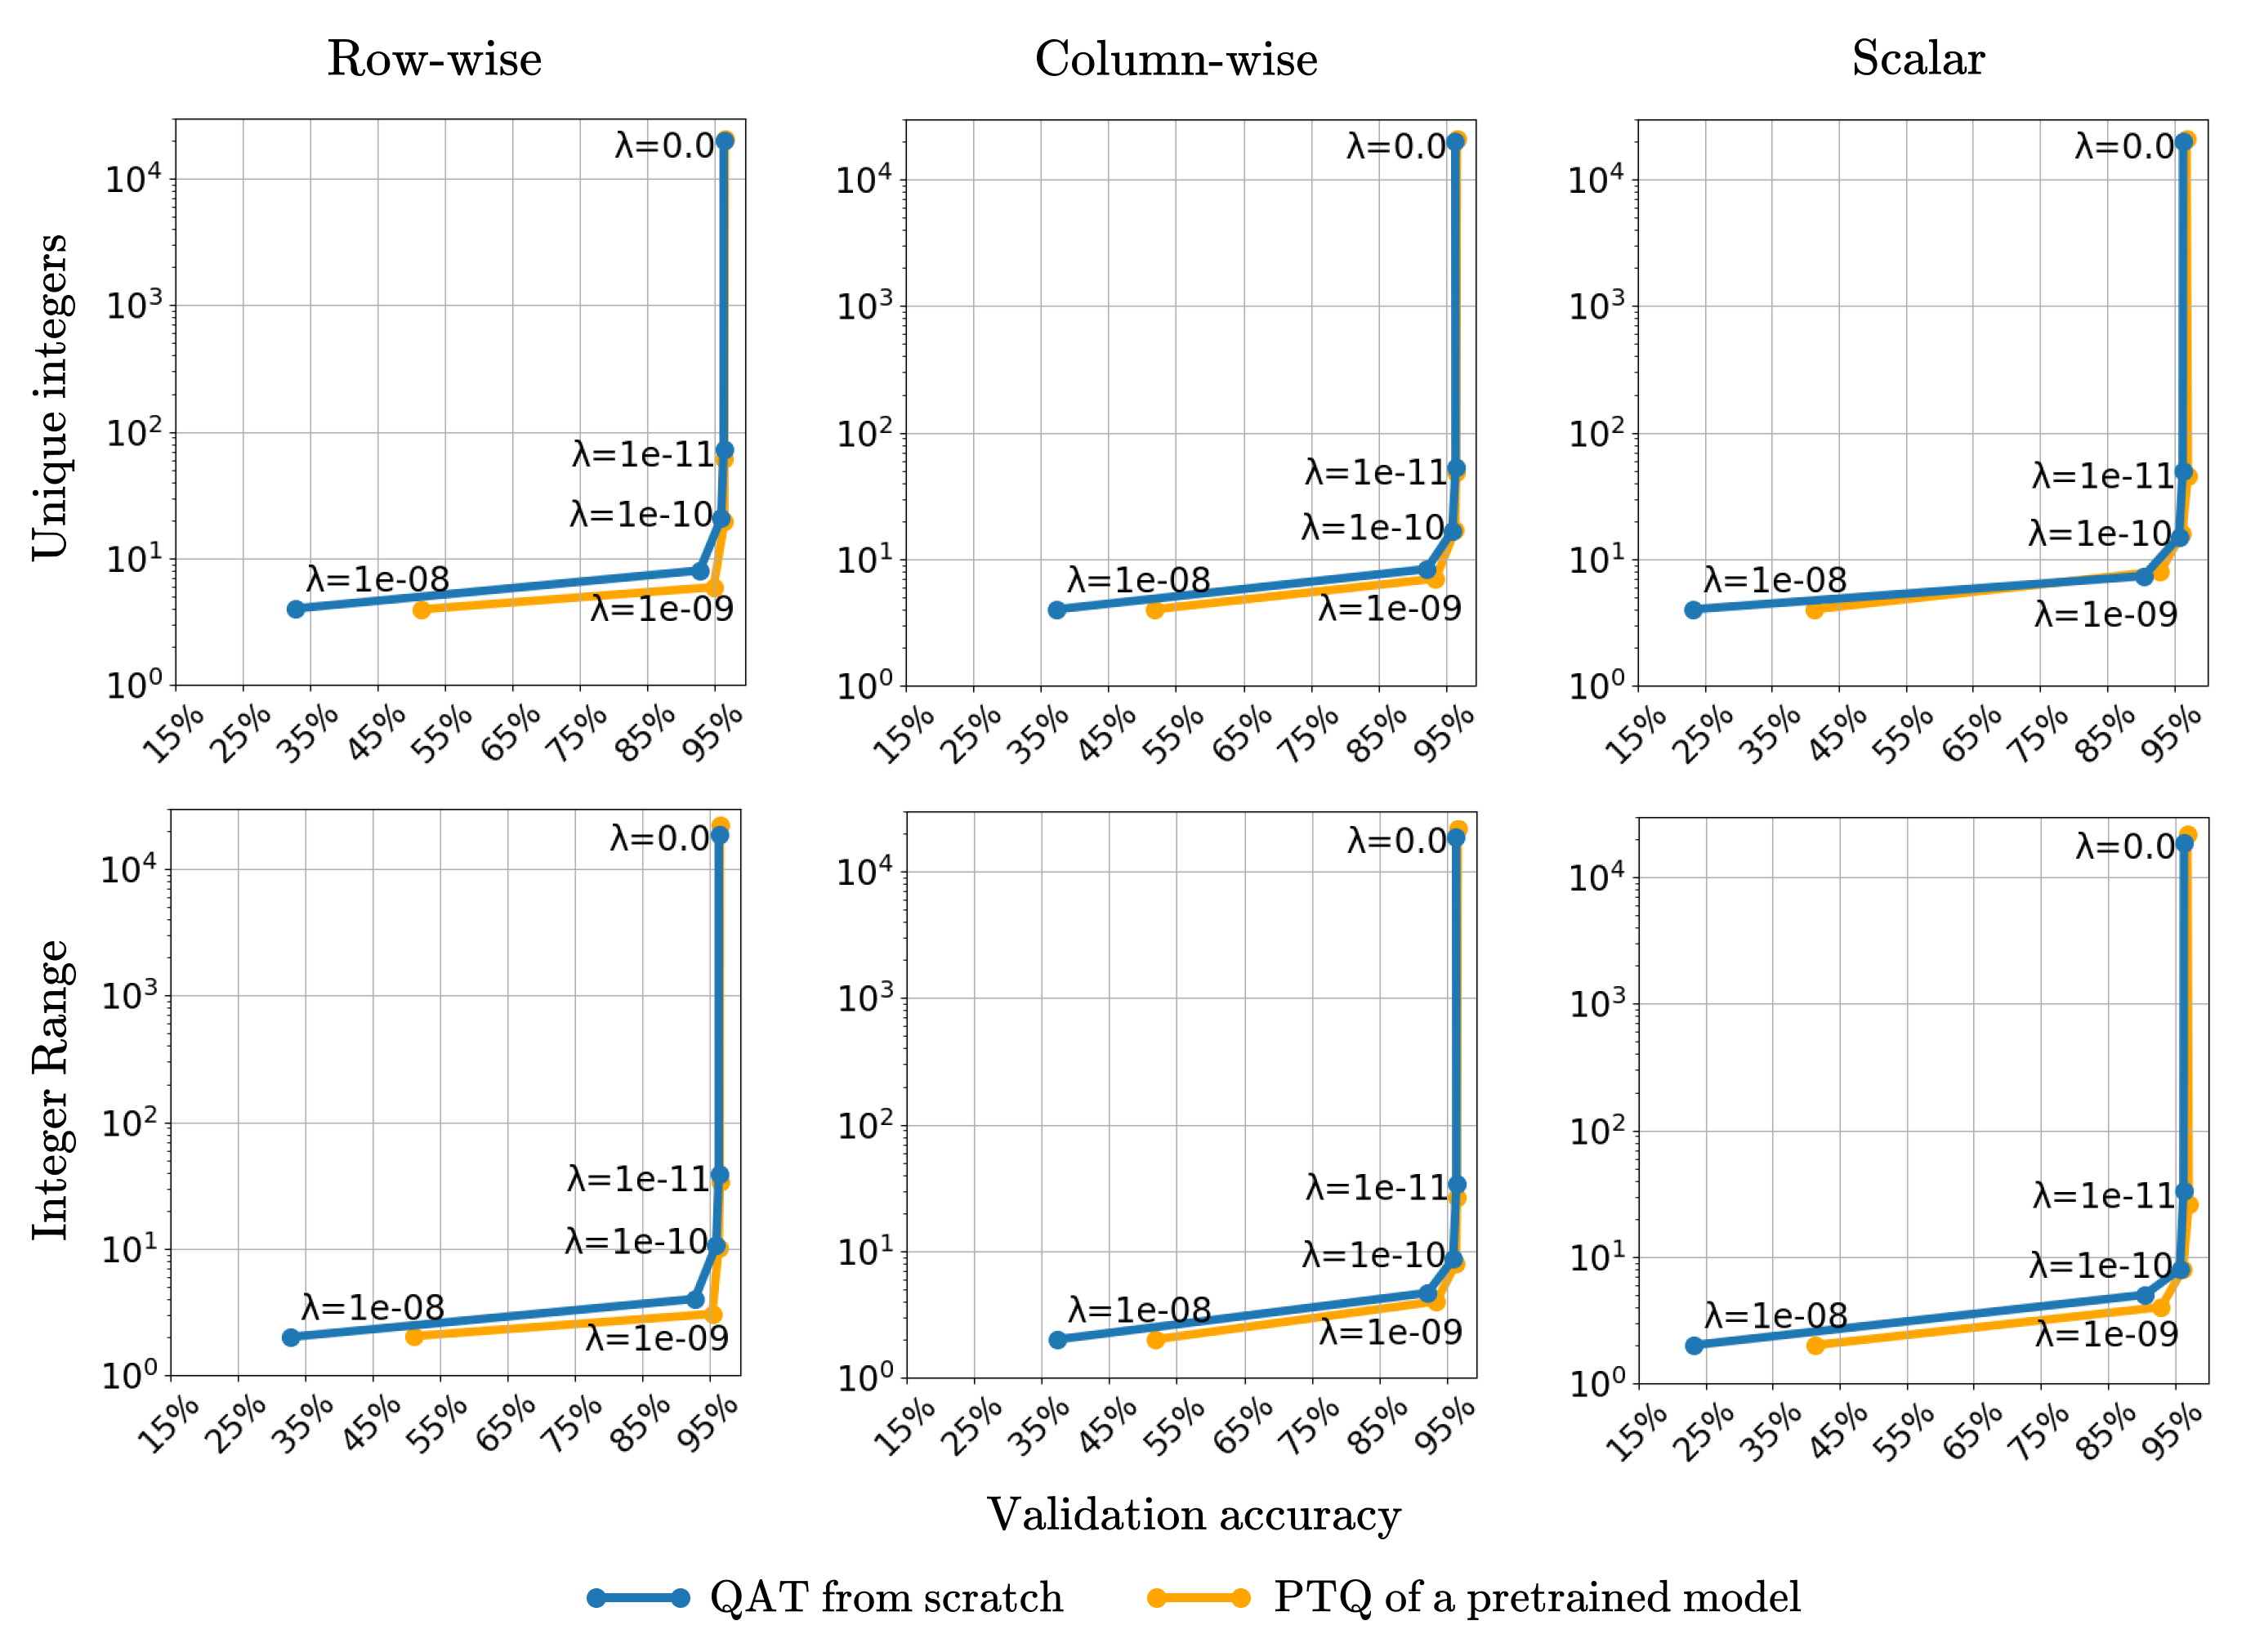
\includegraphics[width=14cm]{pareto-mnist-dense.png}
  \caption{Accuracy – quantization trade-off for nested quantization layers on MNIST.}
  \label{fig:pareto-mnist-dense}
\end{figure}

As an example, the actual integer values after quantization for the row-wise scenario is 
depicted in \cref{fig:quantization_results_1e-10_dense} for all four parameters separately.
While the total number of unique values is only \( 24 \), the range spans from \( -12 \) to \( 11 \).
Consequently, \( 5 \) bits are sufficient to represent the quantized values in the resulting layers, 
as \( \lceil \log_2(24) \rceil = 5 \), covering all 24 unique values within the range. 
The bit requirement can be further reduced using compression techniques like Huffman coding \cite{4051119}, 
considering the concentration of values around 0 in the distributions of quantized weights.


\begin{figure}[b!]
  \centering
  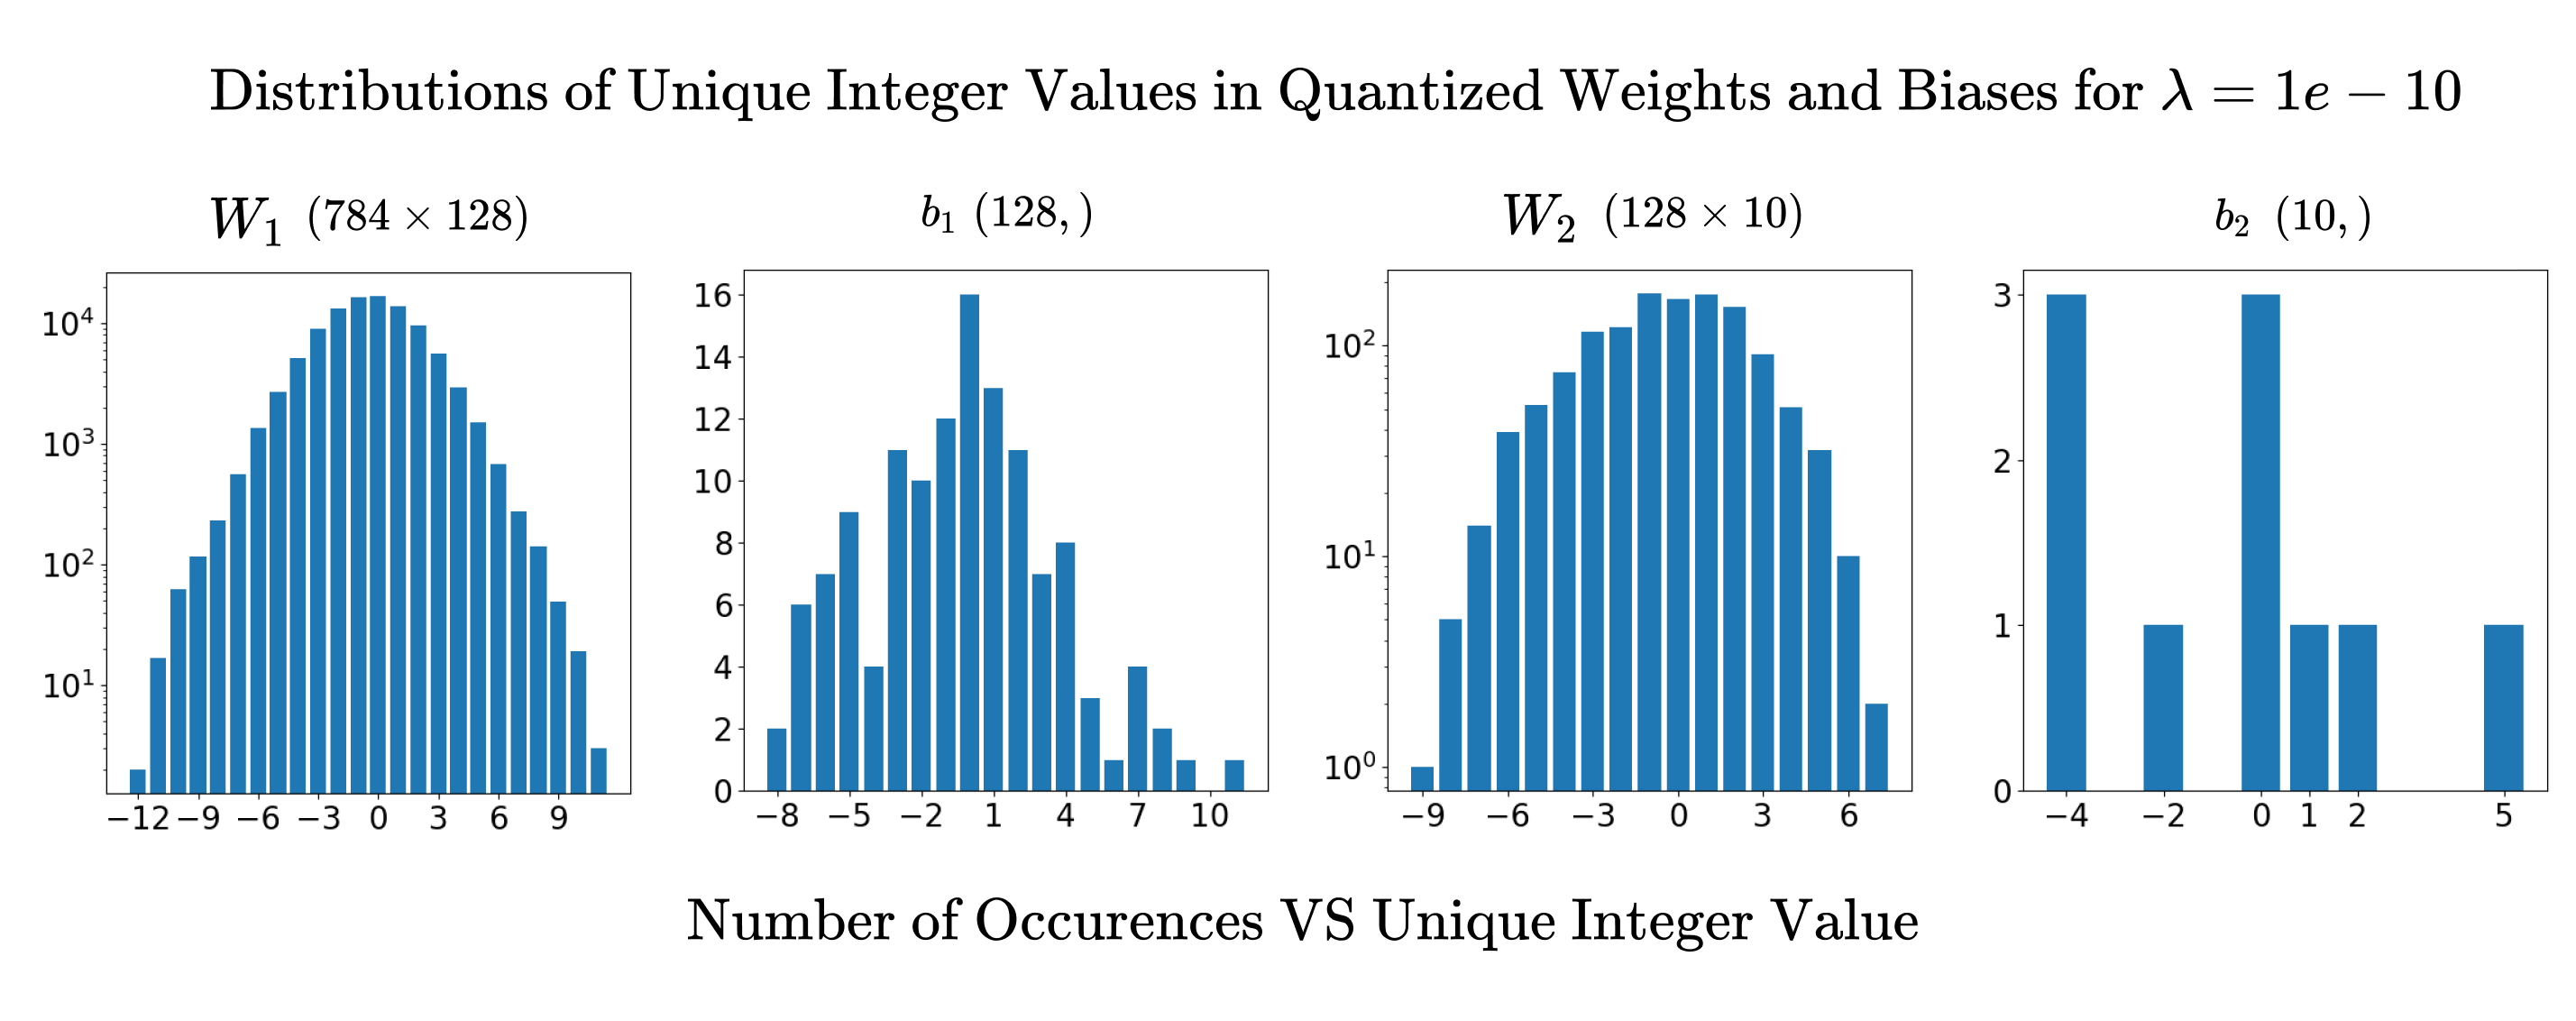
\includegraphics[width=14cm]{quantization_results_1e-10_dense.png}
  \caption{Quantization of MNIST dense layers with row-wise granularity at \( \lambda  = 1e-10 \).}
  \label{fig:quantization_results_1e-10_dense}
\end{figure}


Interestingly, as depicted in \cref{fig:val-accs-over-epochs-dense}, 
the validation loss for \( \lambda = 1e-10 \) 
consistently remains lower than the full-precision baseline and \( \lambda = 0.0 \) throughout the training process.
At the same time, the validation accuracy
remains almost identical to the baseline. This indicates that the penalty threshold of
\( \lambda = 1e-10 \) 
not only preserves the classification accuracy of the model
but also improves generalization with regard to loss,
making the model more confident in its predictions.

\begin{figure}[b!]
  \centering
  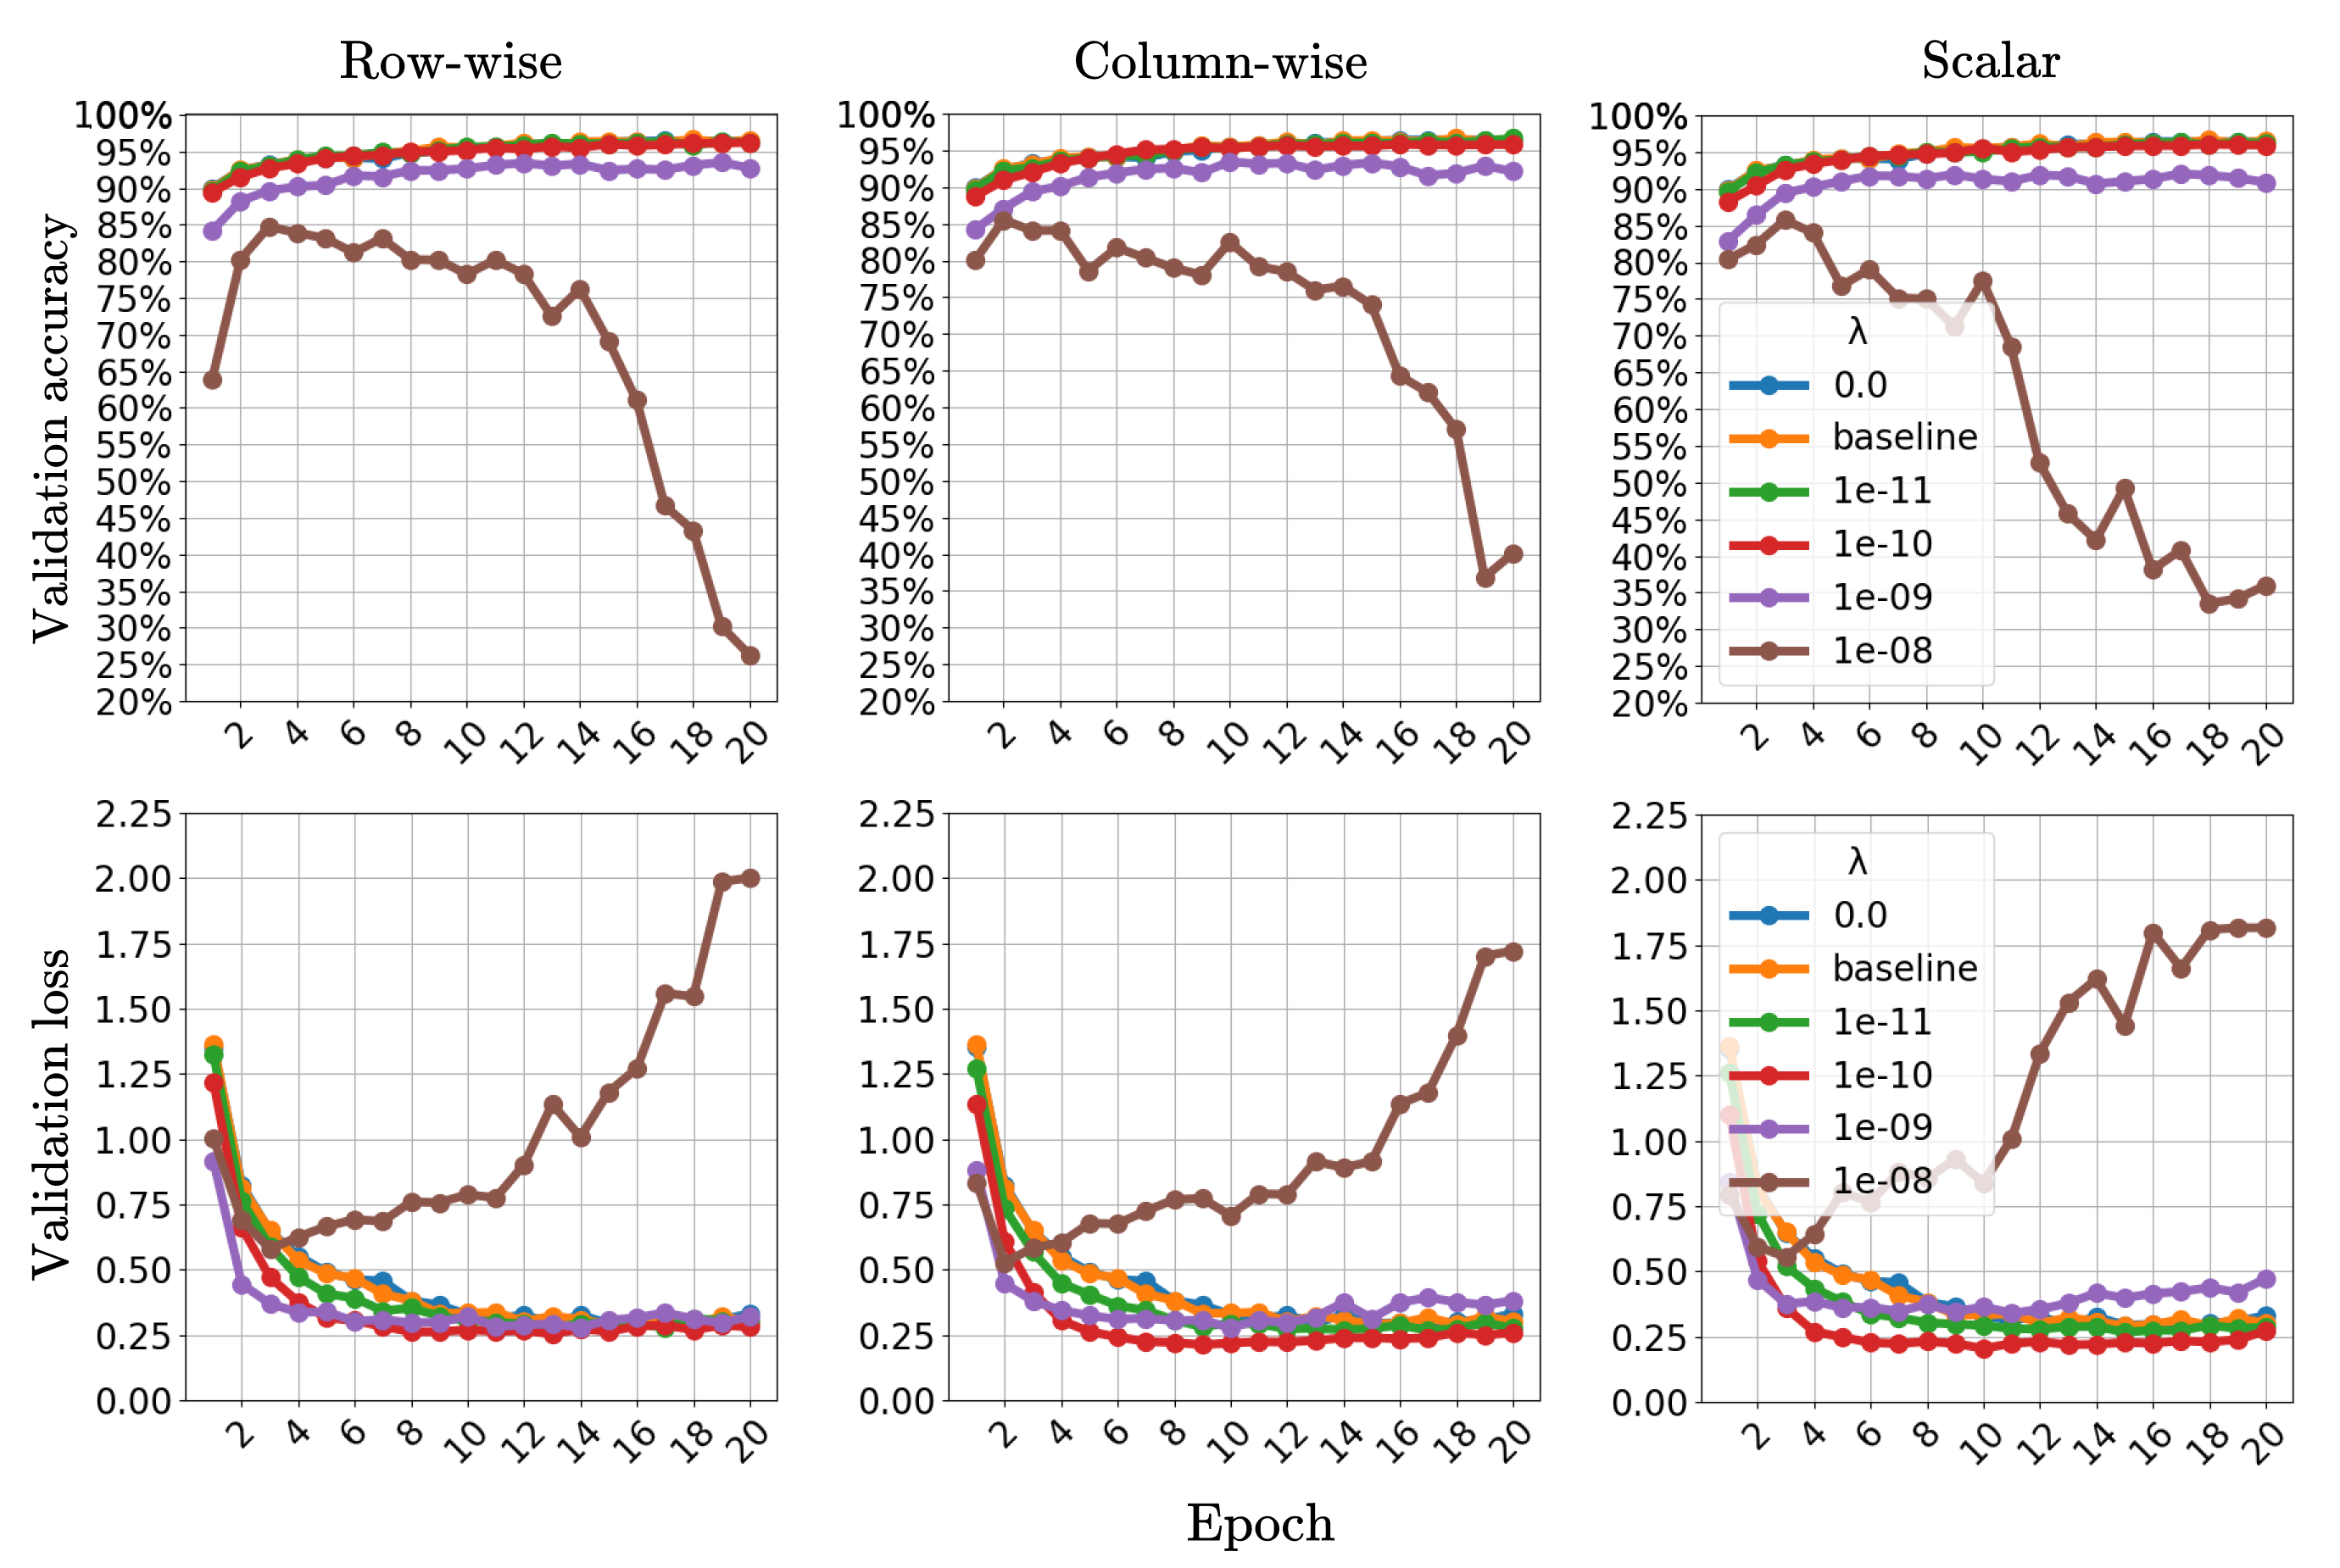
\includegraphics[width=14cm]{dense_nested_val_acc_loss.png}
  \caption{Impact of quantization on accuracy and loss for different \( \lambda \) on MNIST.}
  \label{fig:val-accs-over-epochs-dense}
\end{figure}

In terms of quantization granularity, we see that a scalar scaling factor applied to 
weights produces slightly worse results compared to row-wise and column-wise granularity.
The steeper accuracy degradation and greater loss increase
for \( \lambda = 1e-8\) demonstrate this effect, 
as shown in \cref{fig:val-accs-over-epochs-dense}.
The suboptimal performance of the scalar scaling factor suggests 
that layer-wise quantization, 
which it represents, 
may be too coarse to account for the variability in parameter distributions within a layer.
Therefore, finer granularities, such as row-wise or column-wise scaling, 
are more suitable candidates for optimal quantization granularity of dense layers.

We additionally consider a scenario where the full-precision baseline model is
used to perform post-training quantization (PTQ) with the same set of values for
\( \lambda \). 
In this context, we note that the term PTQ should, in our specific scenario, be extended
to \textit{post-training quantization-aware training}.
However, for simplicity, we continue to use the term PTQ to clearly distinguish this approach from QAT performed from scratch.

As shown
in \cref{fig:pareto-mnist-dense}, we see that the Pareto fronts do not change significantly,
with higher values of \( \lambda \) even achieving a slightly lower number of unique integers at the end
compared to training from scratch.
However, this small advantage is not major. 
As illustrated in \cref{fig:val-accs-over-epochs-dense-pt}, 
this minor benefit occurs only when the model has already lost a significant amount of accuracy.
Nevertheless, the previously defined optimal value of \( \lambda=1e-10 \) holds for PTQ as well,
producing comparable results as shown in \cref{fig:quantization_results_1e-10_dense}

\begin{figure}[b!]
  \centering
  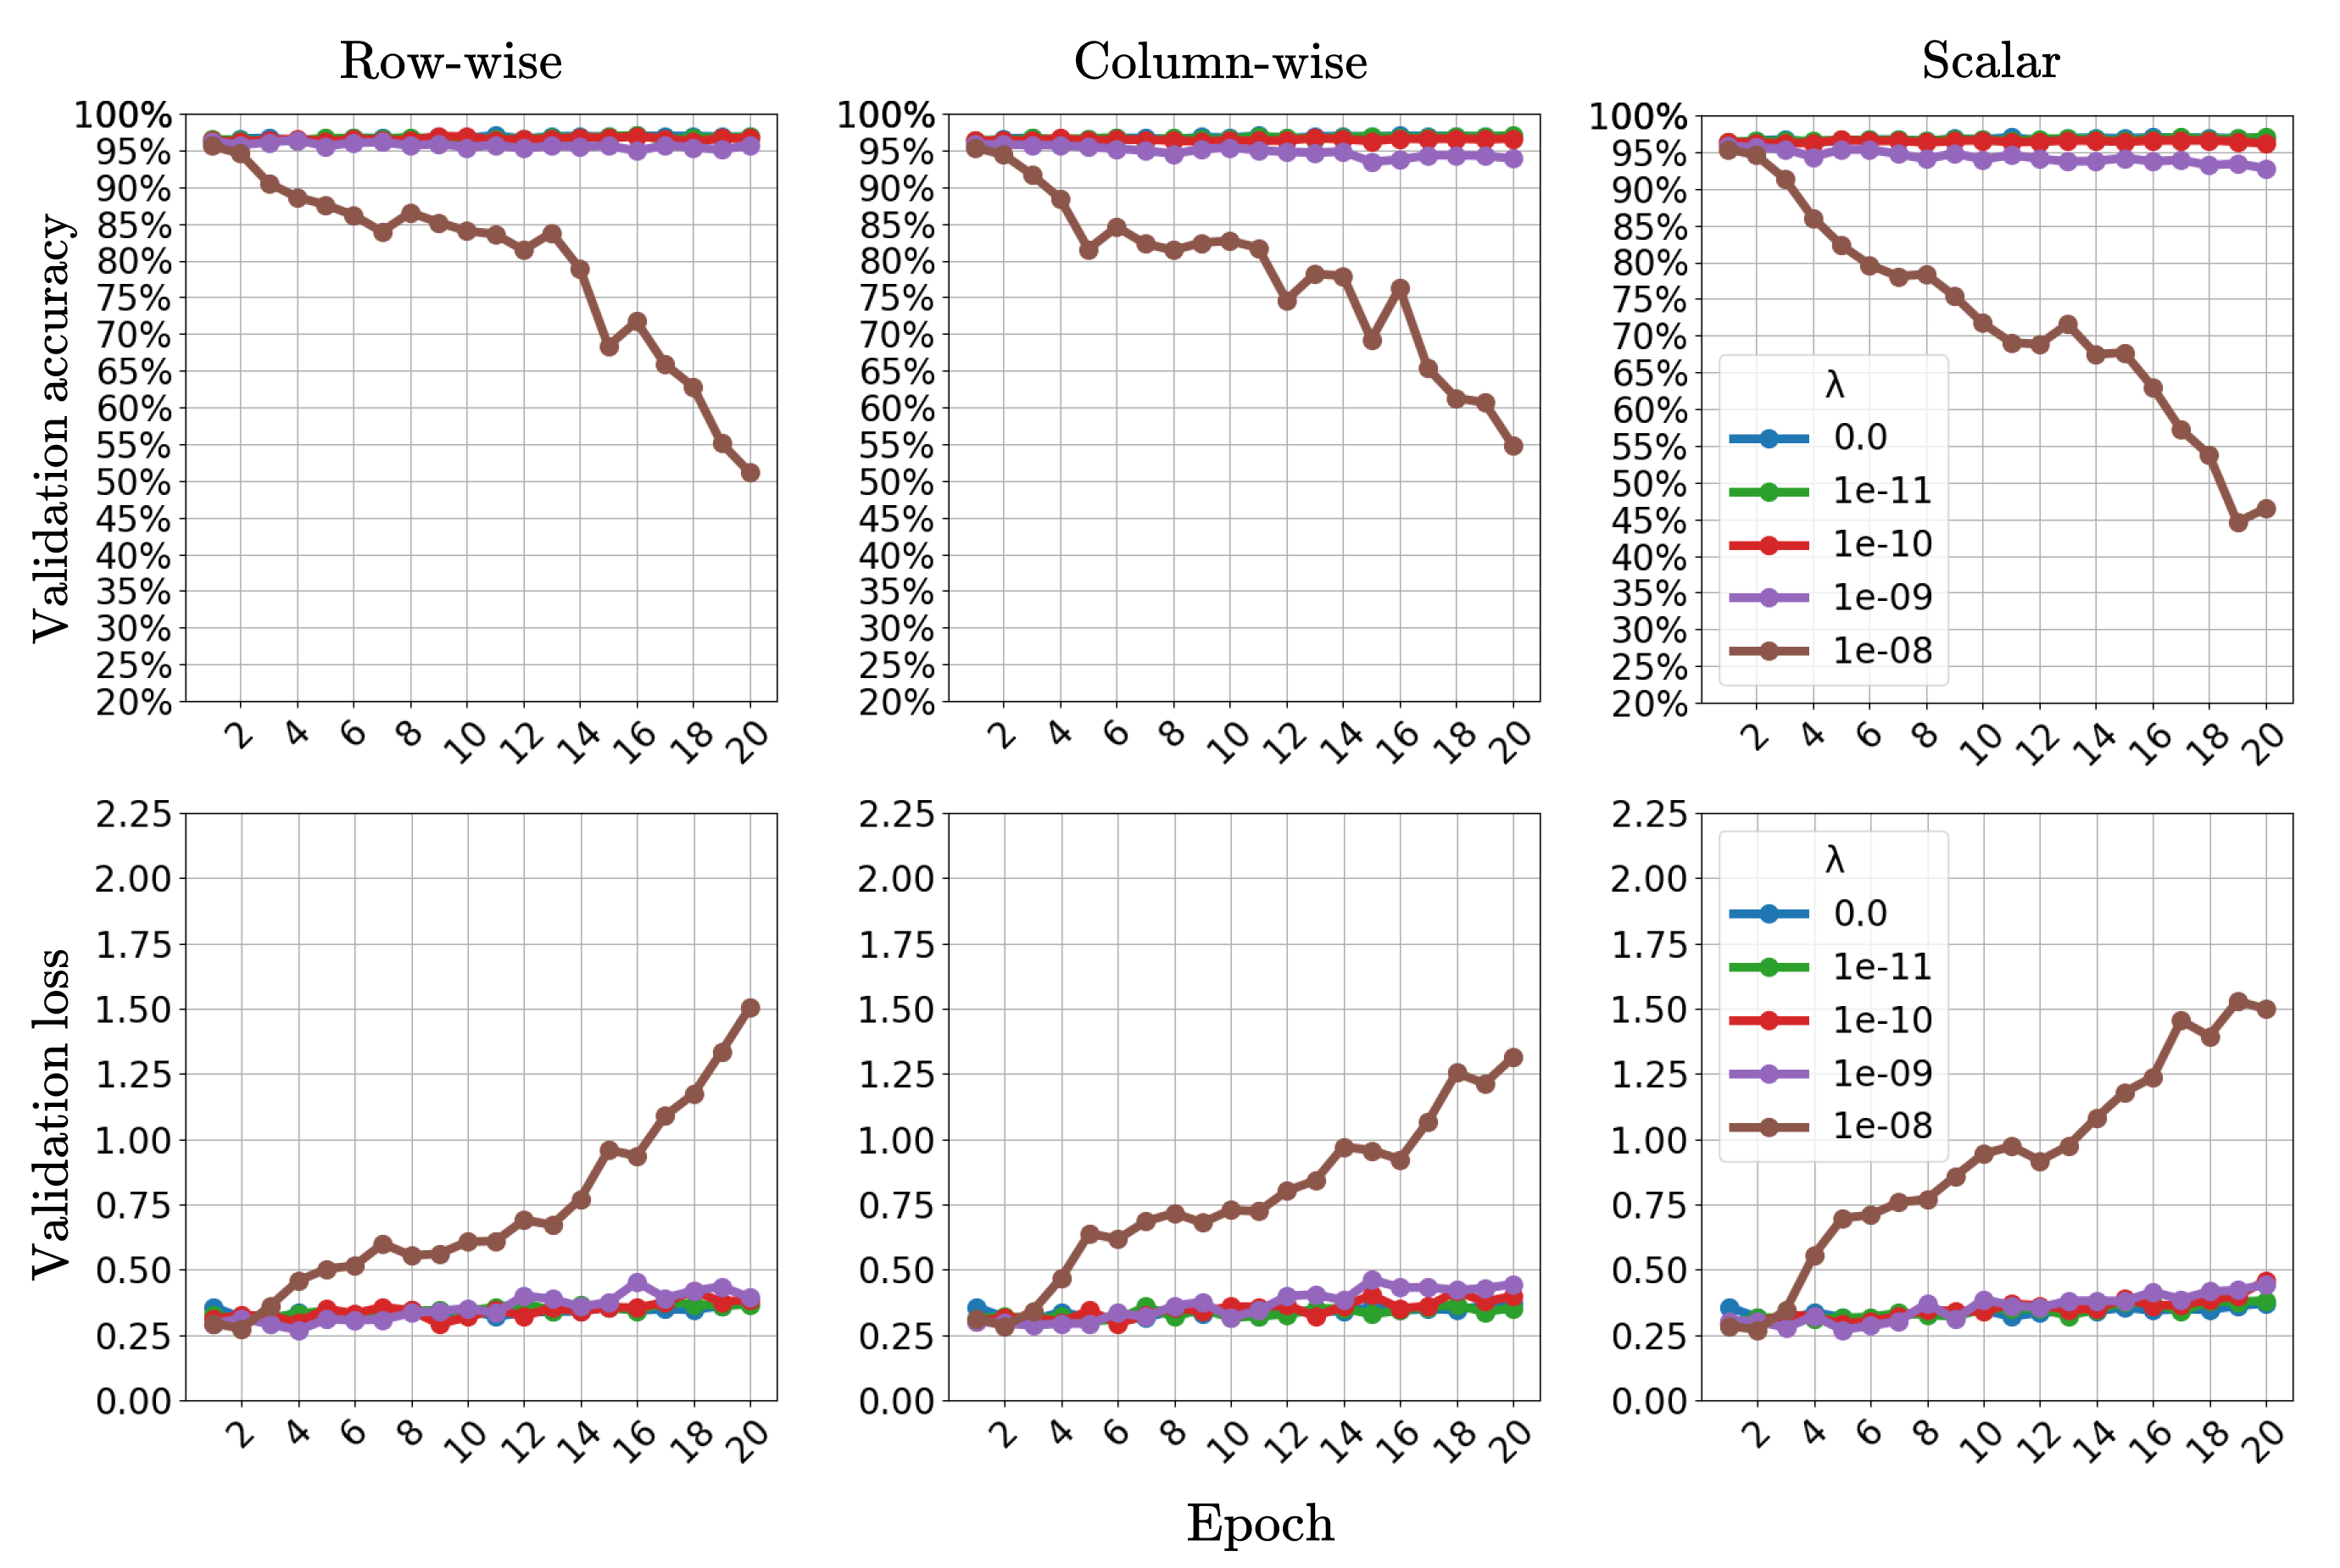
\includegraphics[width=14cm]{dense_nested_val_acc_loss_pt.png}
  \caption{Impact of PTQ on accuracy and loss for different \( \lambda \) on MNIST.}
  \label{fig:val-accs-over-epochs-dense-pt}
\end{figure}

% ----------------------- Nested conv ----------------------- 

\subsection{Convolutional Layers}
\label{subsec:convolutionallayers}
\hspace*{1em}For the CIFAR-10 dataset, we define a CNN, with six nested convolutional layers. 
Each convolutional layer has a kernel and a bias. We examine four scenarios:
applying the scale factor channel-wise, row-wise, column-wise, and as a single
scalar for the entire kernel. For all scenarios, a scalar factor is used for each 
bias vector, similar to how we quantized dense layers. The kernel configurations are shown in
\cref{tab:scalefactorgranularityconv} for clarity.

\begin{table}[t!]
  \centering
  \scriptsize
  \caption{Scale factor granularity for convolutional kernels}
  \label{tab:scalefactorgranularityconv}
  \begin{tabular}{lcccc}
    \toprule
    \textbf{Kernel}                      & \textbf{Channel-wise} & \textbf{Row-wise} & \textbf{Column-wise} & \textbf{Scalar} \\ 
    \midrule
    \( K_{1} \) \( (3, 3, 3, 32) \)     & \( (1, 1, 3, 1) \) & \( (3, 1, 1, 1) \) & \( (1, 3, 1, 1) \) & \( (1, 1, 1, 1) \) \\ 
    \( K_{2} \) \( (3, 3, 32, 32) \)    & \( (1, 1, 32, 1) \) & \( (3, 1, 1, 1) \) & \( (1, 3, 1, 1) \) & \( (1, 1, 1, 1) \) \\ 
    \( K_{3} \) \( (3, 3, 32, 64) \)    & \( (1, 1, 32, 1) \) & \( (3, 1, 1, 1) \) & \( (1, 3, 1, 1) \) & \( (1, 1, 1, 1) \) \\ 
    \( K_{4} \) \( (3, 3, 64, 64) \)    & \( (1, 1, 64, 1) \) & \( (3, 1, 1, 1) \) & \( (1, 3, 1, 1) \) & \( (1, 1, 1, 1) \) \\ 
    \( K_{5} \) \( (3, 3, 64, 128) \)   & \( (1, 1, 64, 1) \) & \( (3, 1, 1, 1) \) & \( (1, 3, 1, 1) \) & \( (1, 1, 1, 1) \) \\ 
    \( K_{6} \) \( (3, 3, 128, 128) \)  & \( (1, 1, 128, 1) \) & \( (3, 1, 1, 1) \) & \( (1, 3, 1, 1) \) & \( (1, 1, 1, 1) \) \\ 
    \bottomrule
  \end{tabular}
  \vspace{0.5em}
  \caption*{\footnotesize Note: \( (1, 1, 1, 1) \) denotes a scalar, broadcasted across the kernel for consistency.}
\end{table}

The experiments show that the optimal value for the hyperparameter is \( \lambda = 1e-11\),
across all four scenarios, as depicted in \cref{fig:pareto-cifar-conv}.
\begin{figure}[b!]
  \centering
  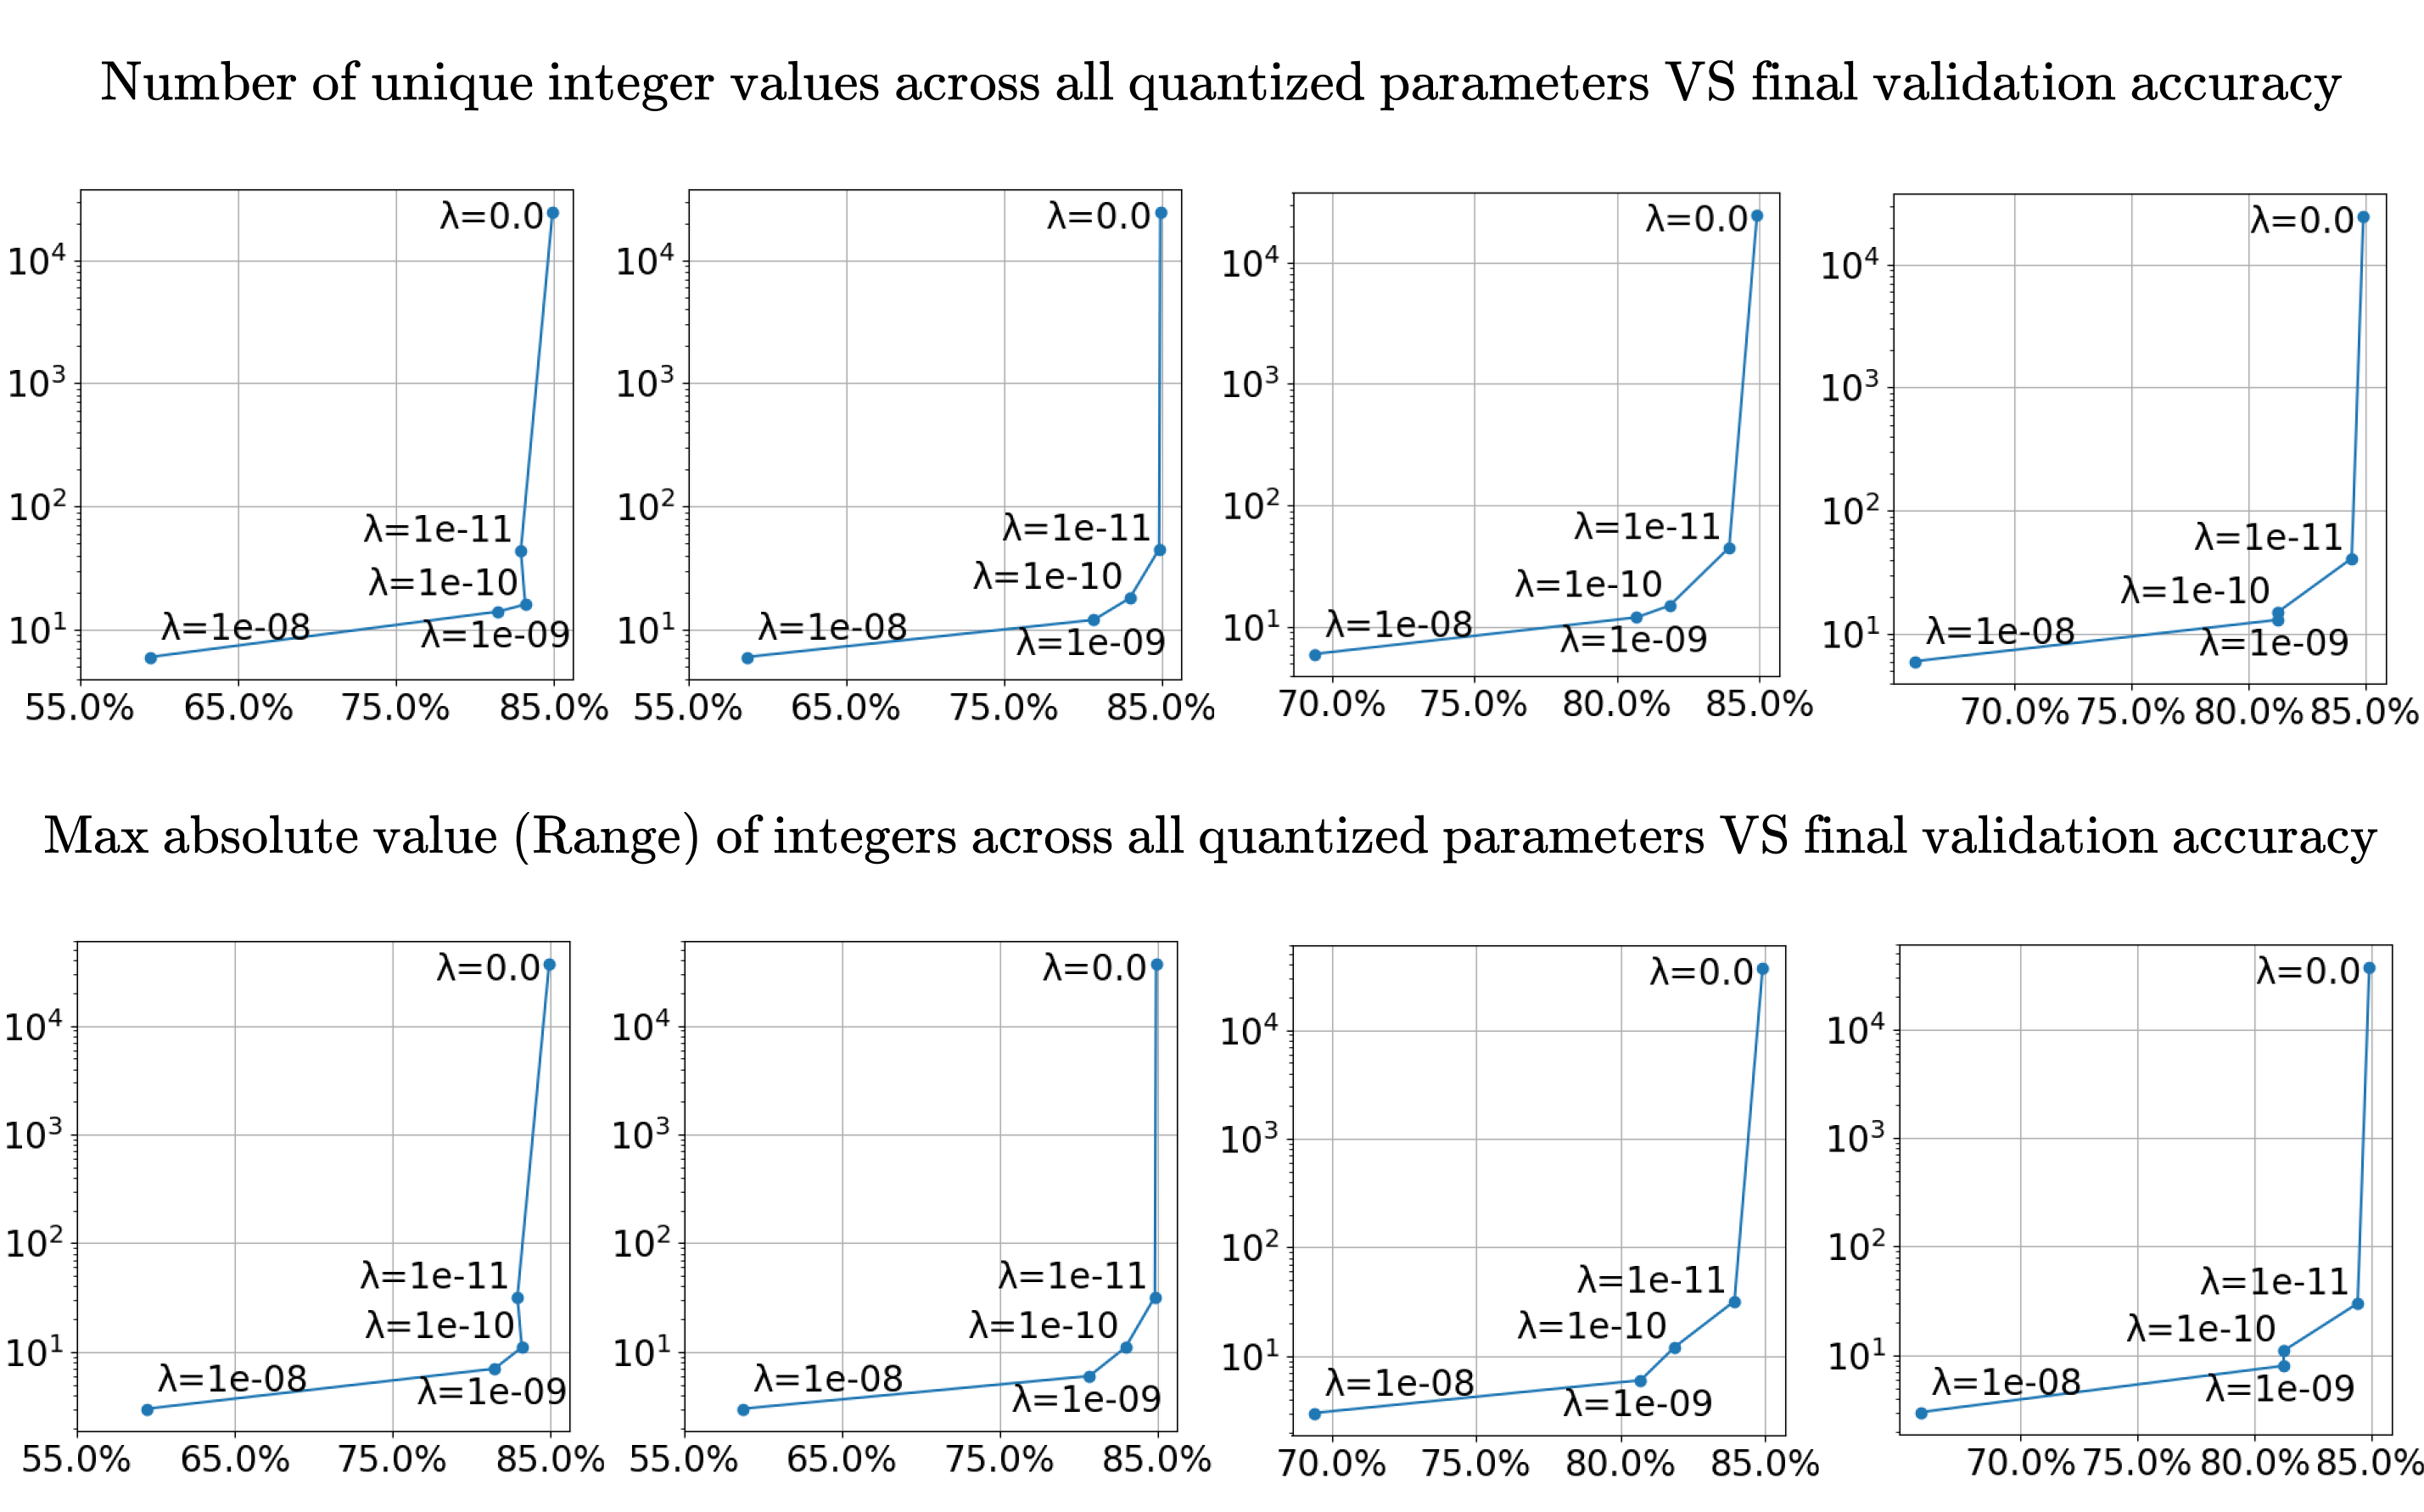
\includegraphics[width=14cm]{pareto-cifar-conv.png}
  \caption{Accuracy–quantization trade-off for nested quantization layers on CIFAR-10.}
  \label{fig:pareto-cifar-conv}
\end{figure}
As an example, the integer values after quantization for the row-wise scenario across
all quantized parameters range from \( -22 \) to \( 32 \), 
resulting in \( 60 \) unique values that can be represented with \( \lceil \log_2(60) \rceil = 6 \) bits.
The histograms of the resulting integer values in the kernels, displayed in \cref{fig:quantization-results-1e-10conv},
form a bell curve similar to the experimental results for dense layer weights.
\begin{figure}[t!]
  \centering
  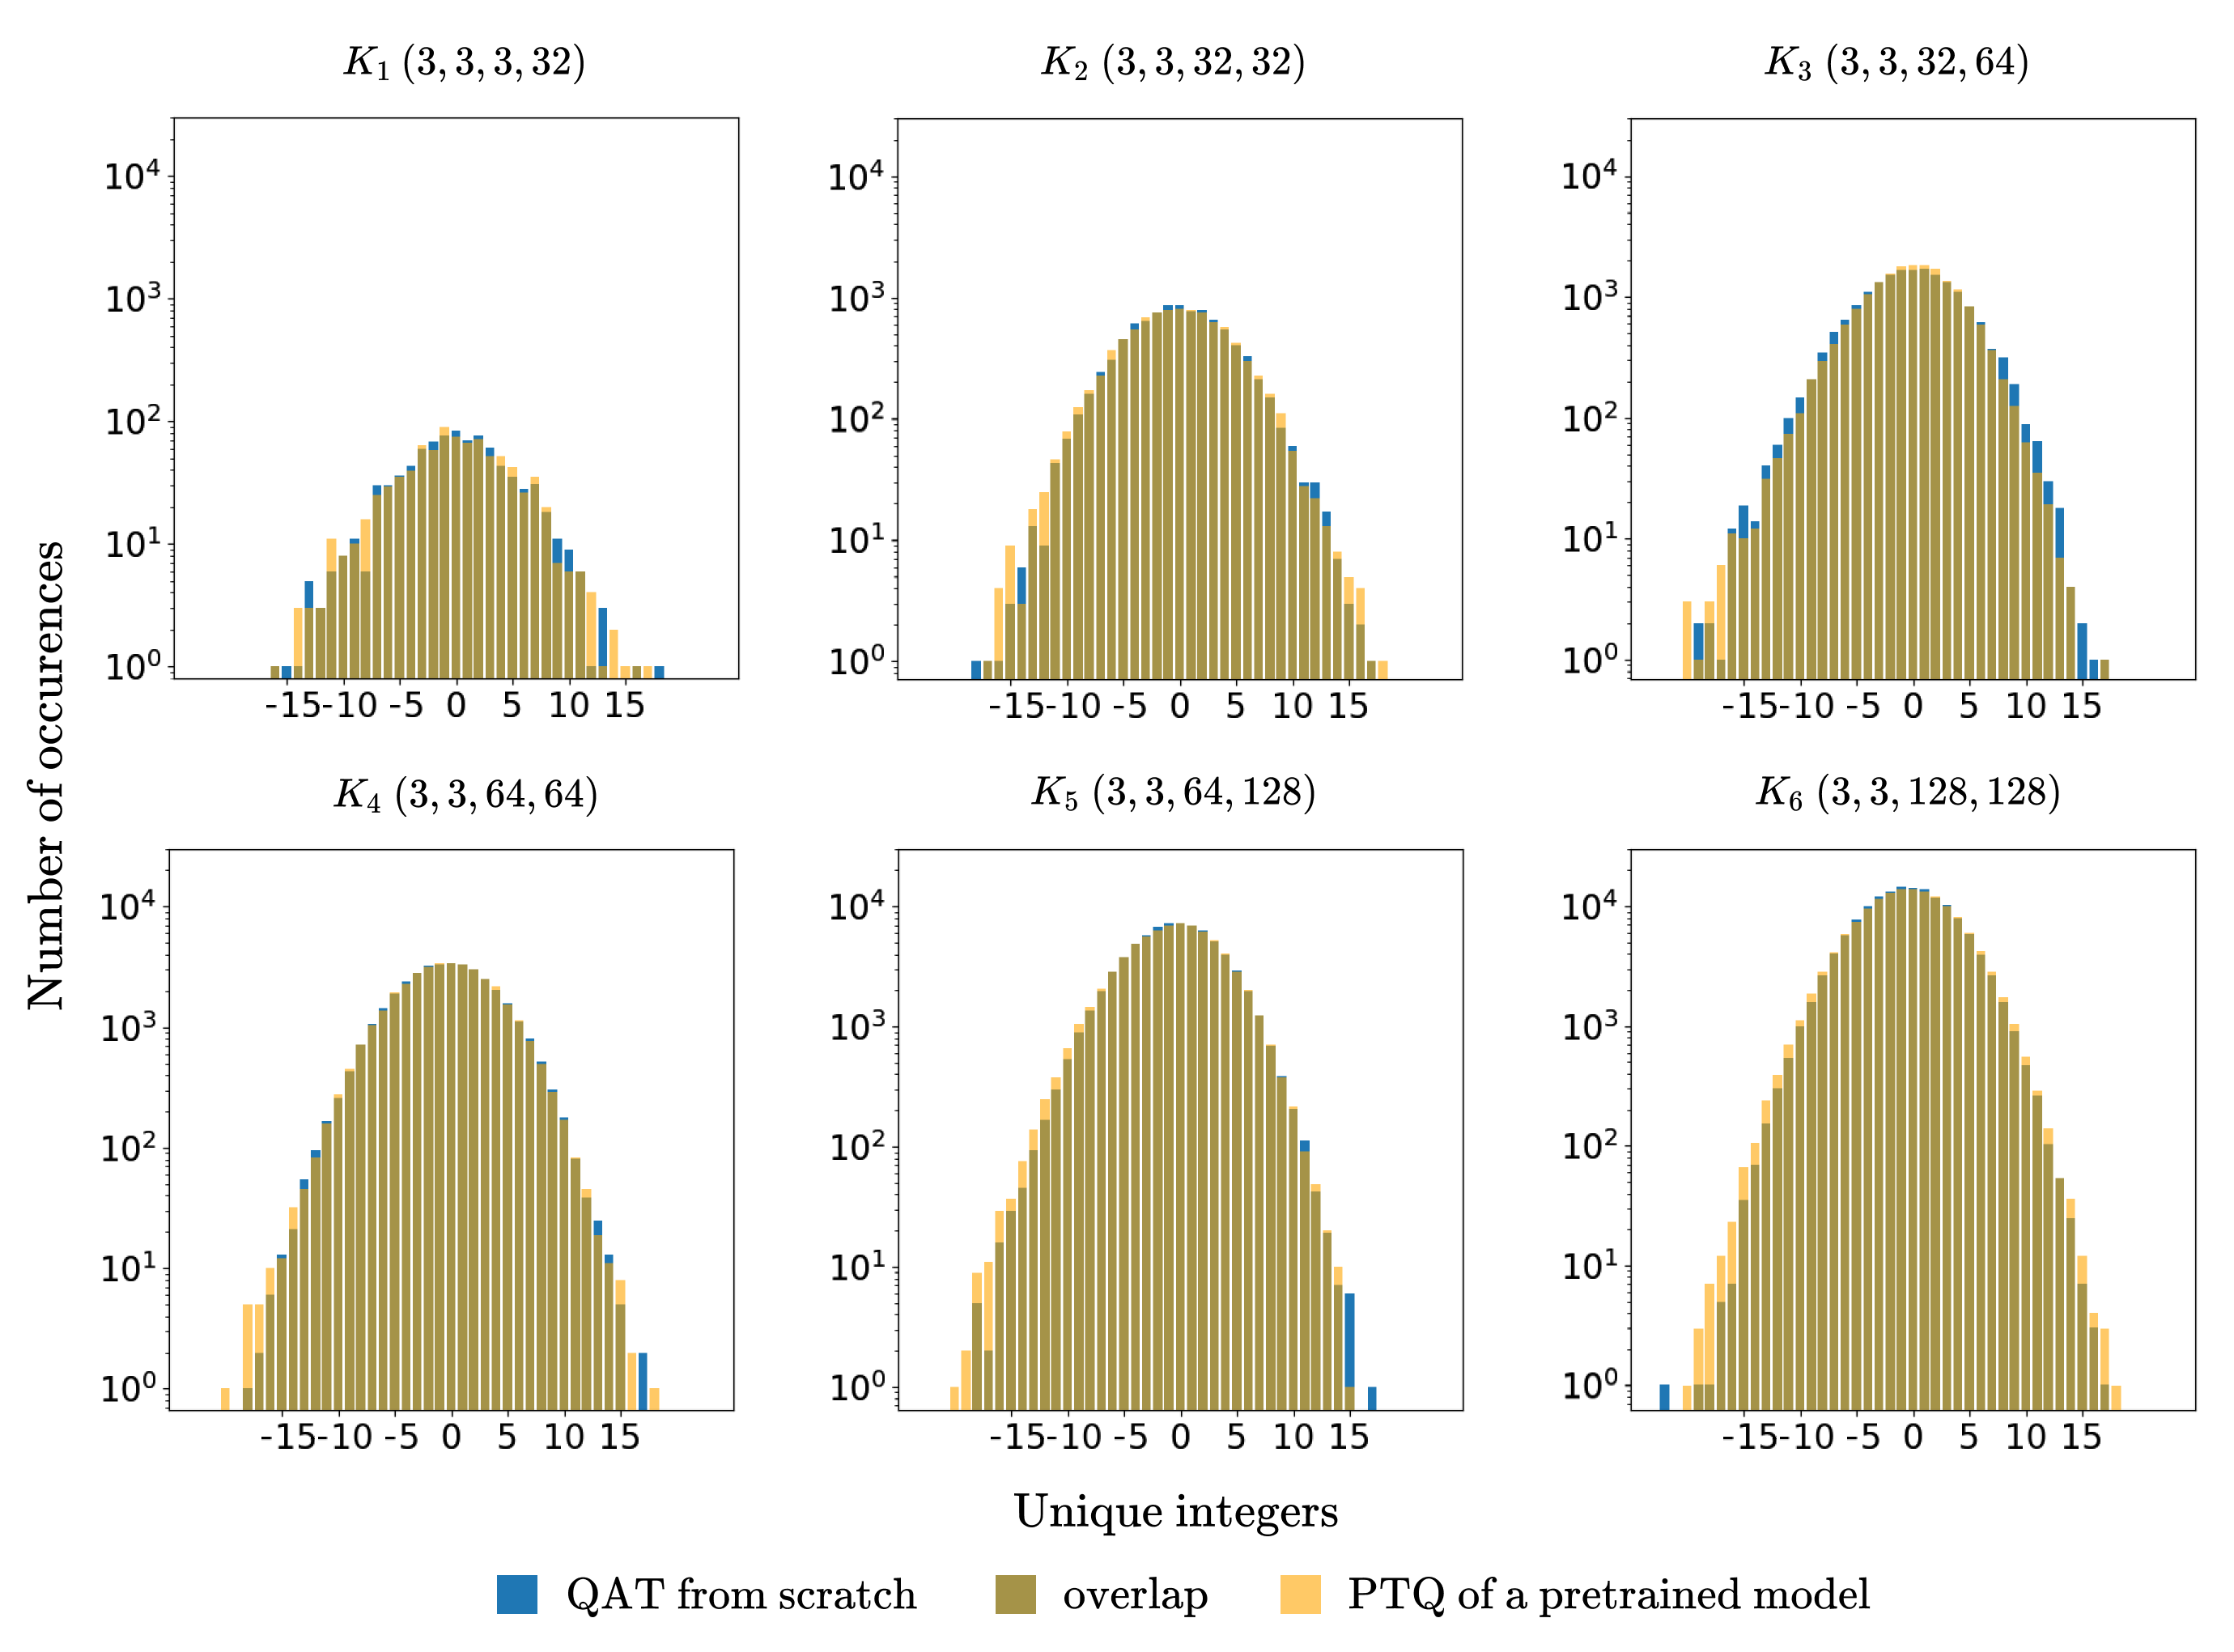
\includegraphics[width=14cm]{quantization_results_1e-11_conv.png}
  \caption{Quantization of CIFAR-10 kernels with row-wise granularity at  \( \lambda  = 1e-11 \).}
  \label{fig:quantization-results-1e-10conv}
\end{figure}
\begin{figure}[t!]
  \centering
  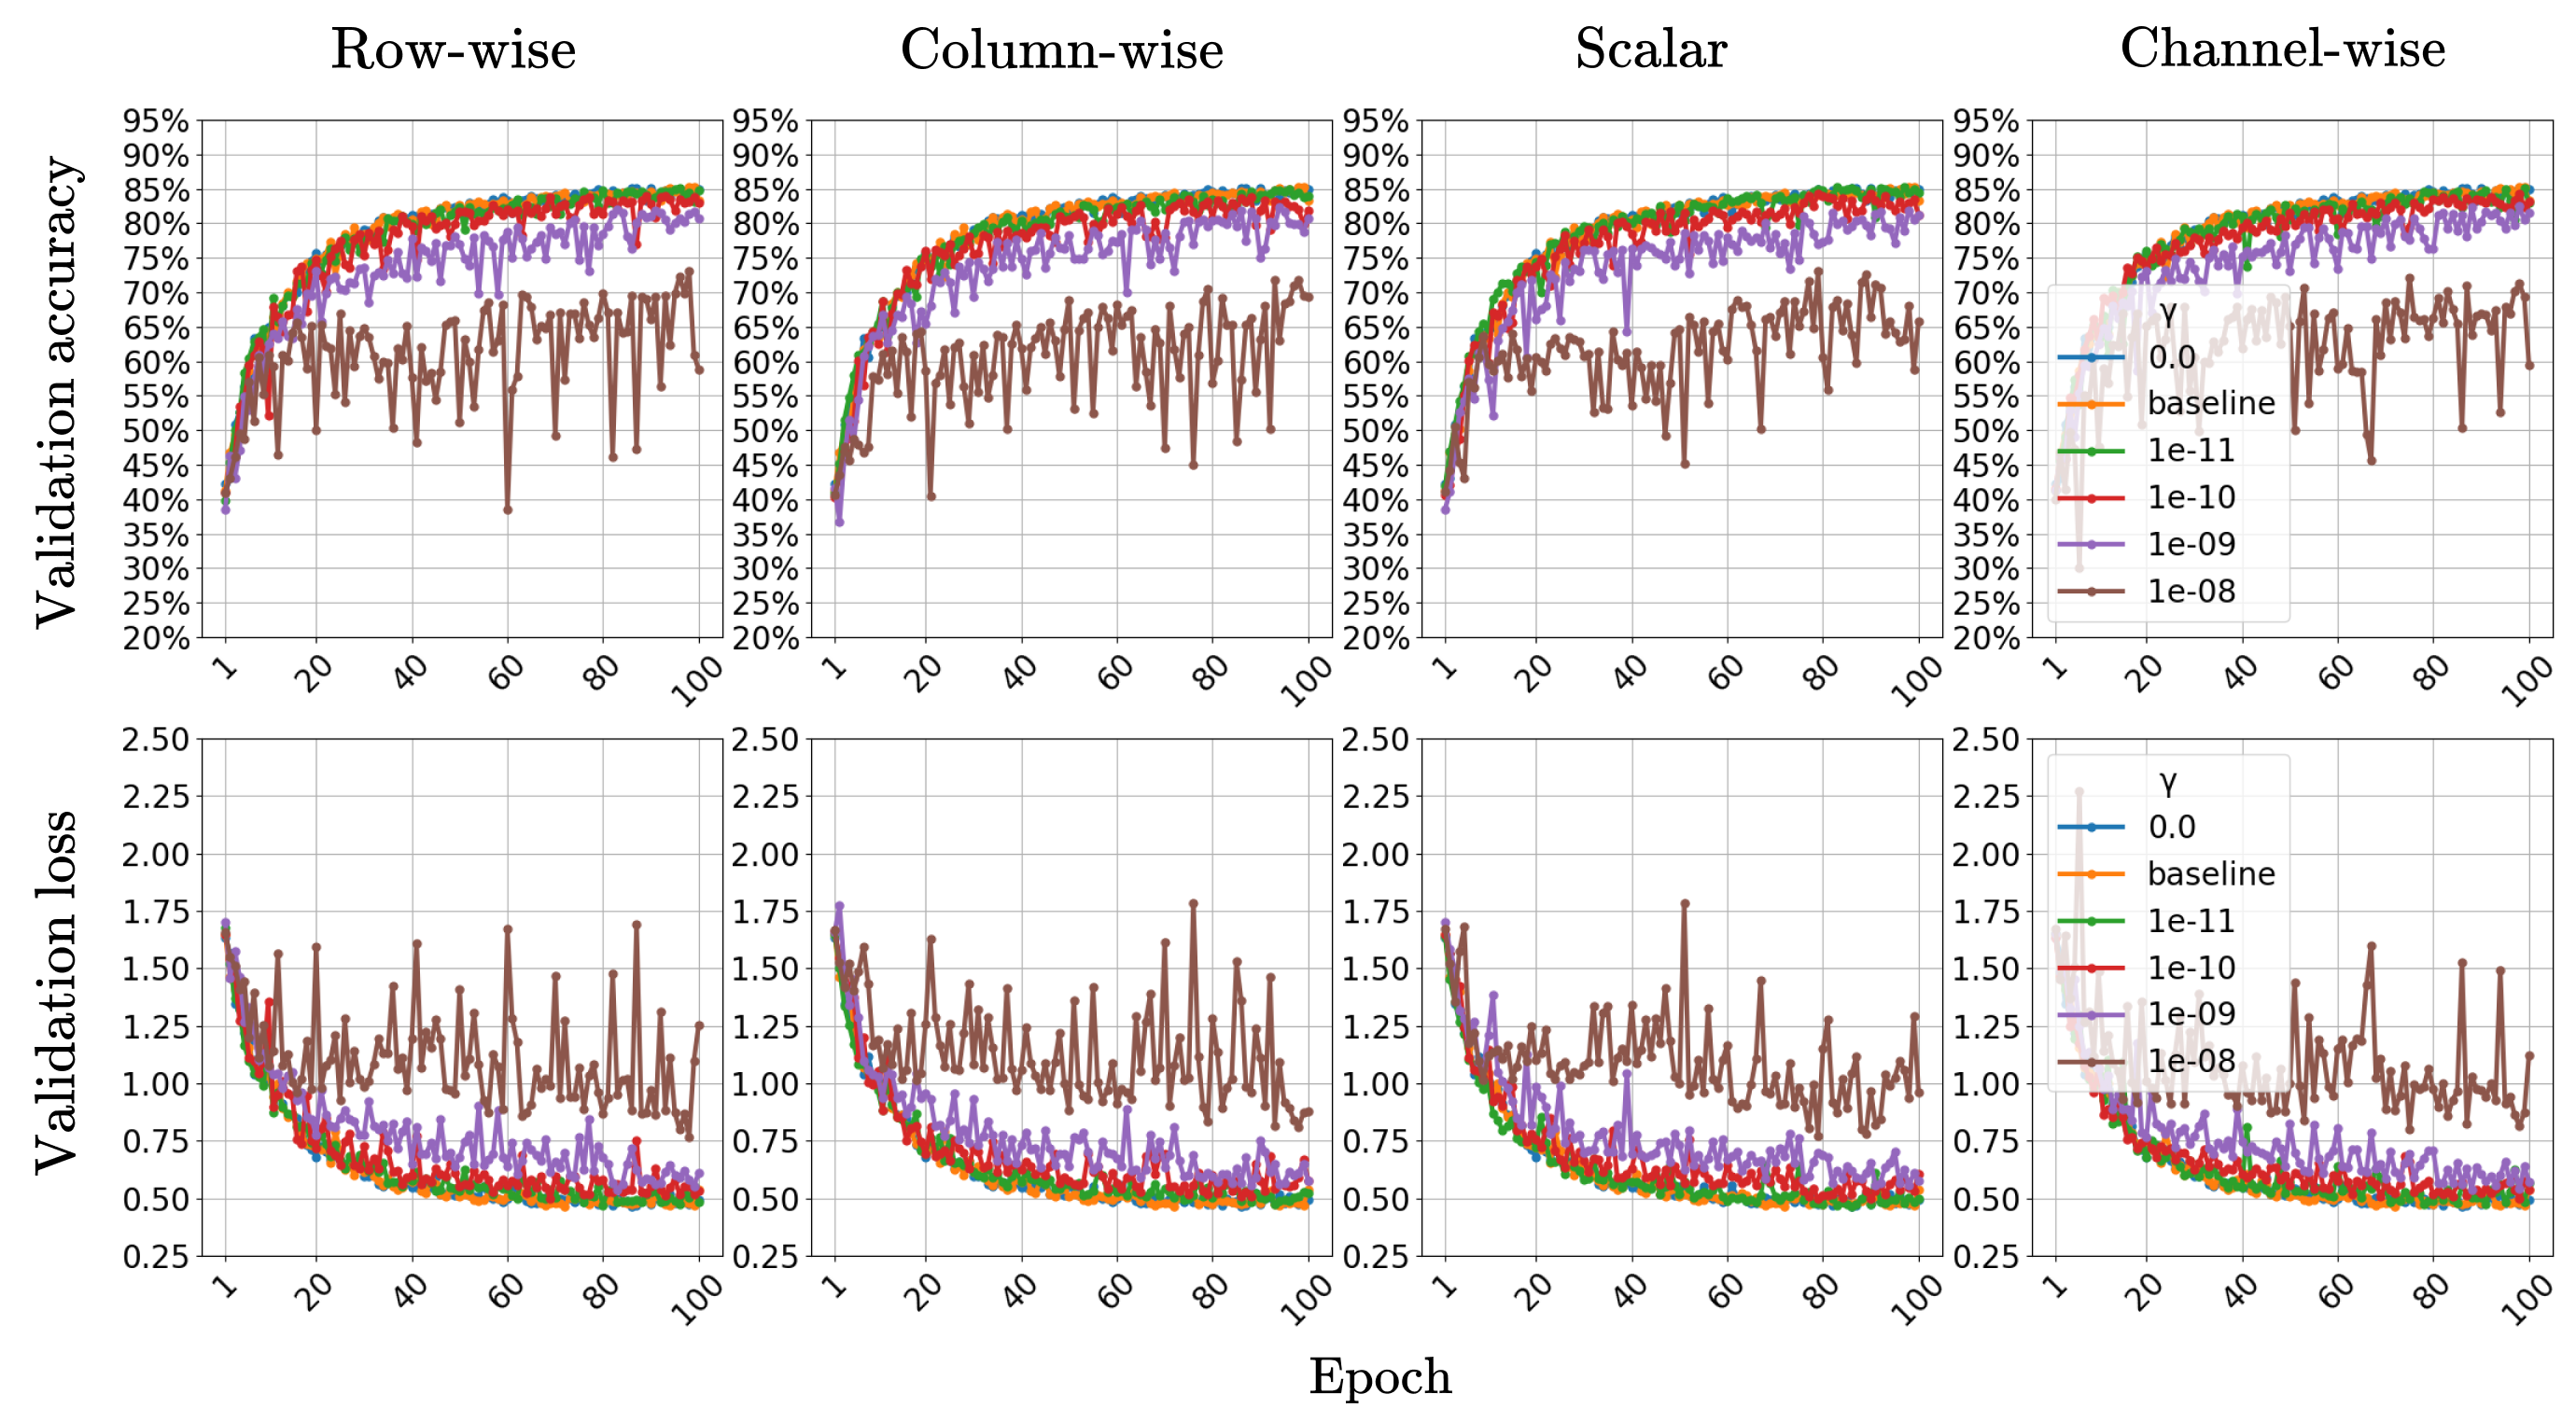
\includegraphics[width=14cm]{conv_nested_val_acc_loss.png}
  \caption{Impact of quantization on accuracy and loss for different \( \lambda \) on CIFAR-10.}
  \label{fig:val-accs-over-epochs-conv}
\end{figure}
If a slightly greater degradation in accuracy is viable, 
\( \lambda \) can be increased to \( \lambda = 1e-10\).
In the row-wise case, this adjustment results in a reduced range of integers,
spanning from \( -8 \) to \( 11 \). Further increasing \( \lambda \) could
reduce the number of unique values to less than 10.

\begin{table}[b!]
  \centering
  \caption{Compression rate of the nested quantization layer method}
  \label{tab:nestedcomrpessionrate}
  \begin{tabular}{lccc}
      \toprule
      \textbf{Dataset}     & \textbf{Baseline} & \textbf{PTQ + Compression} & \textbf{Granularity, $\lambda$} \\ 
      \midrule
      MNIST                & $\approx 0.36 $ MB            & $\approx 0.05 $ MB              & row-wise, $1e-10$         \\ 
      CIFAR-10          &  $\approx 1.02 $ MB          & $\approx 0.16 $ MB            & row-wise, $1e-11$            \\ 
      Imagenette               &  $\approx 39.57 $ MB          & $\approx 6.39 $ MB             & channel-wise, $1e-11$          \\ 

      \bottomrule
  \end{tabular}
  \vspace{0.5em}
\end{table}


\begin{figure}[t!]
  \centering
  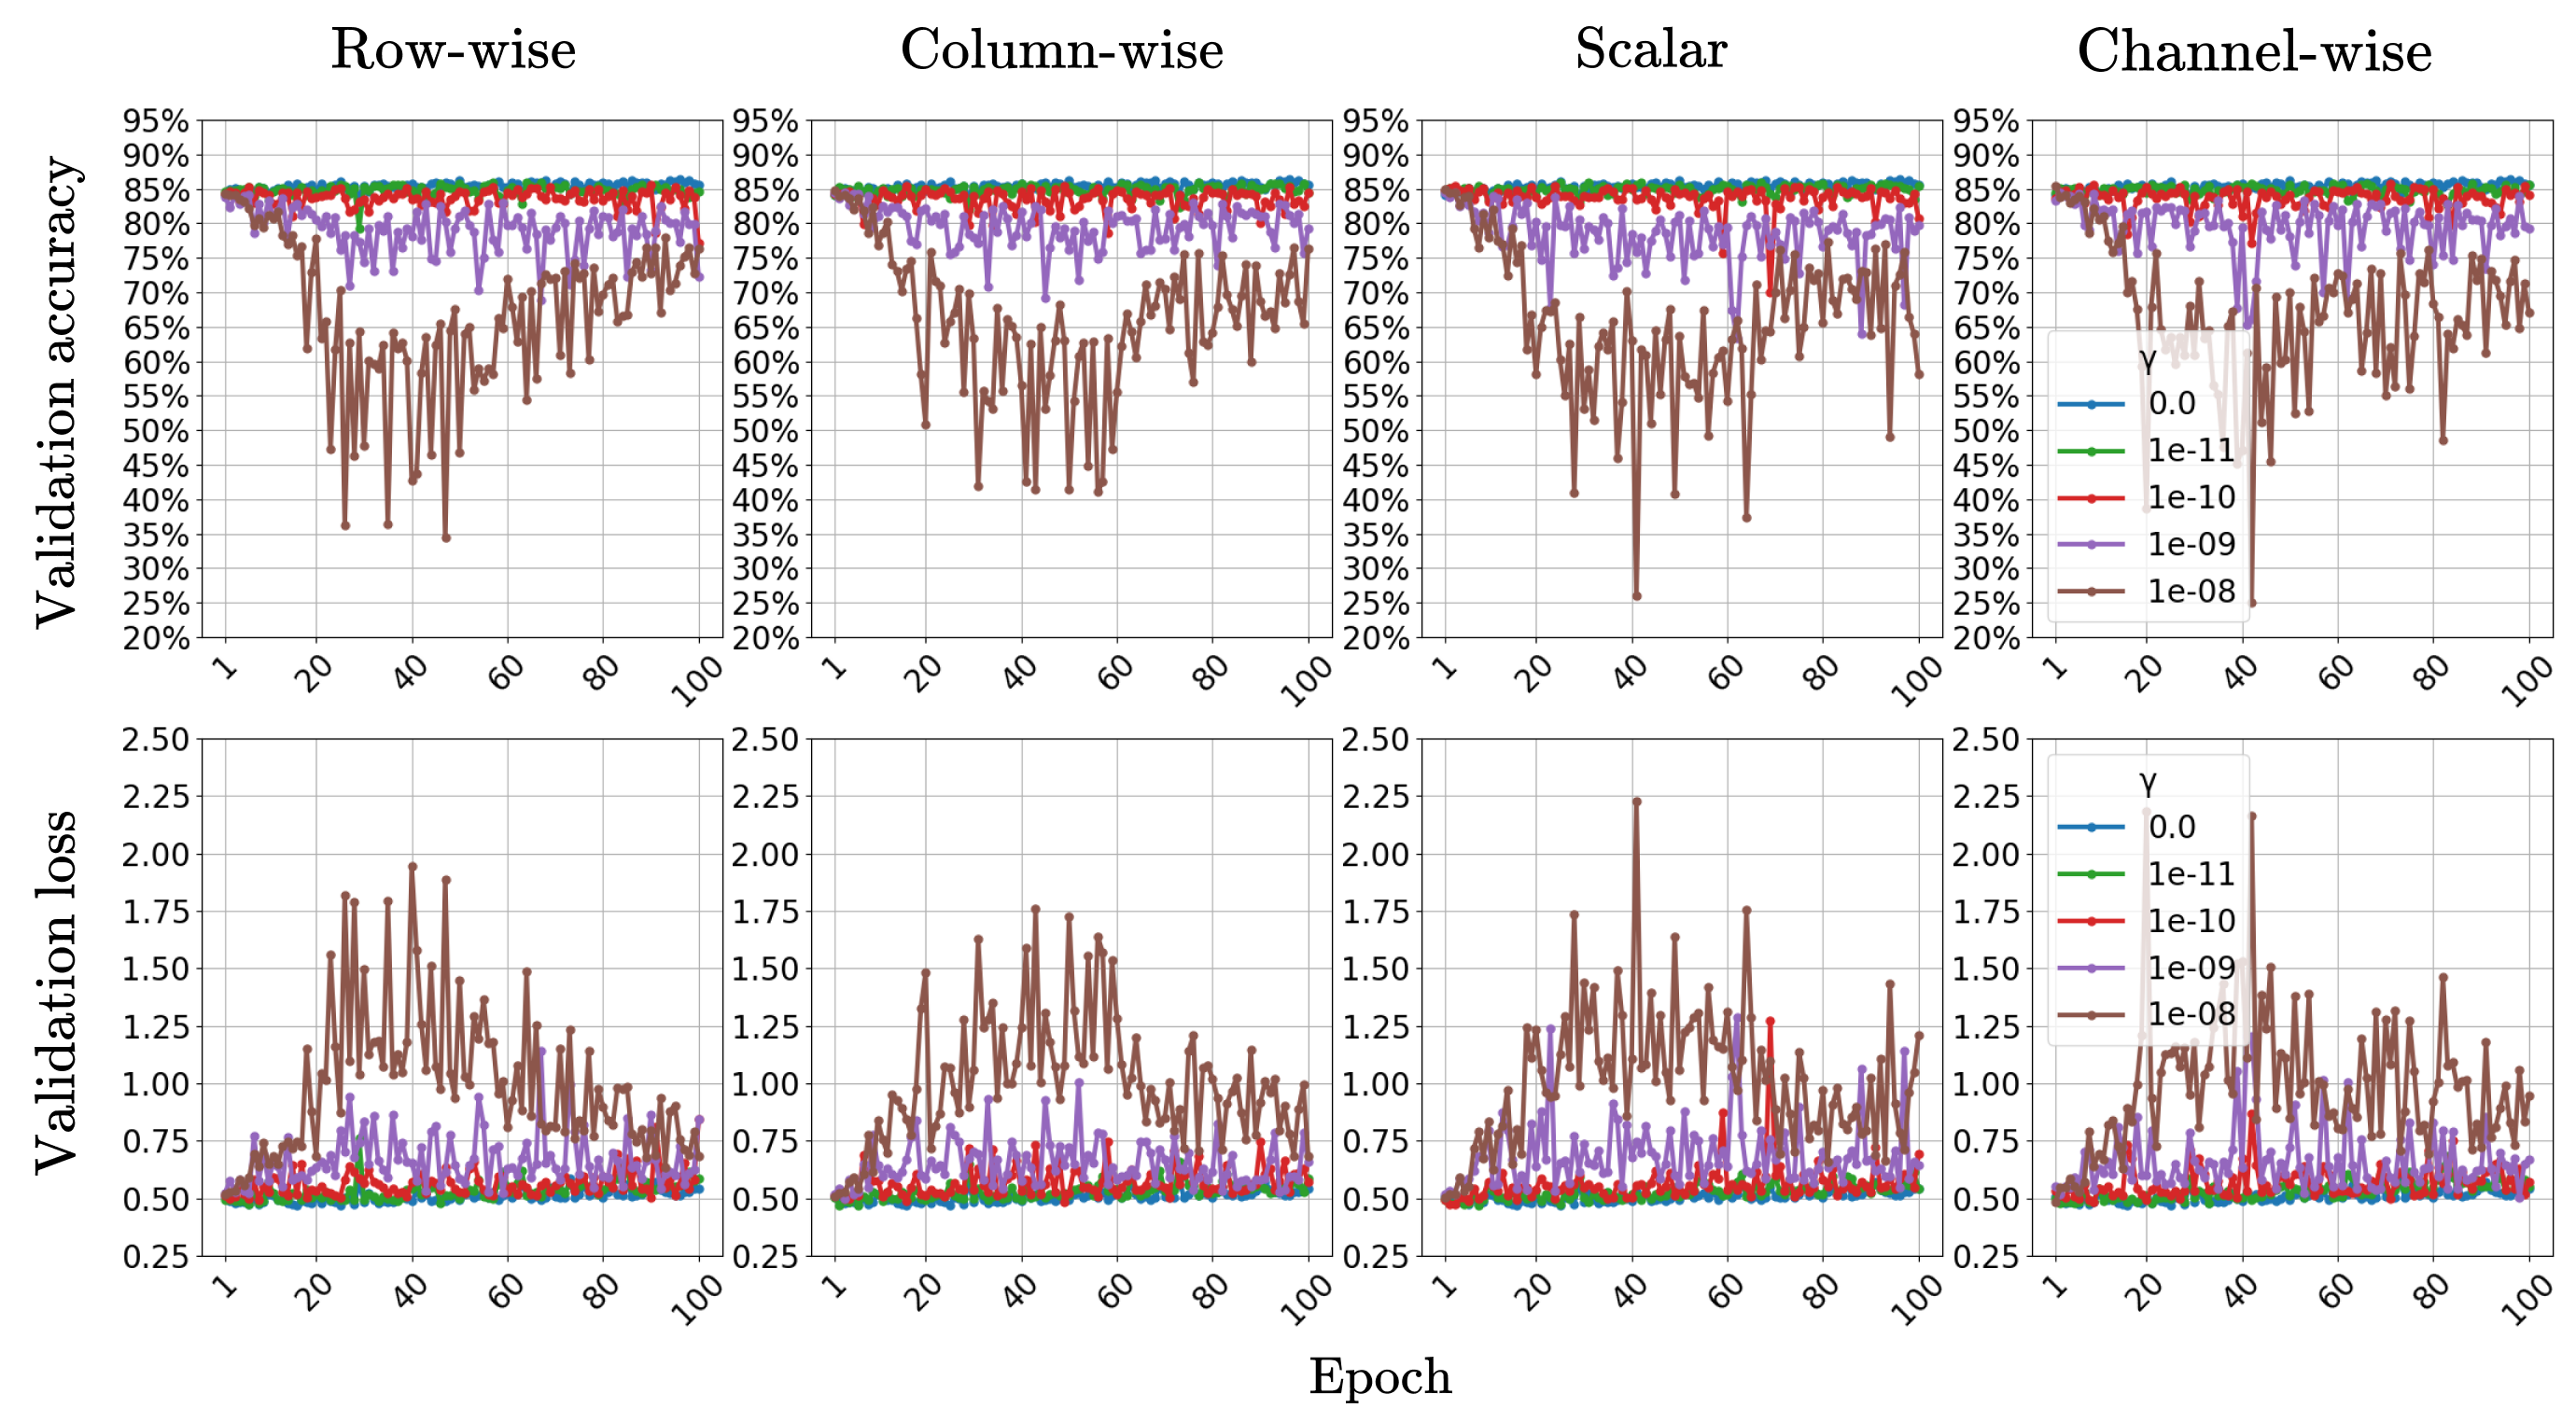
\includegraphics[width=14cm]{conv_nested_val_acc_loss_pt.png}
  \caption{Impact of PTQ on accuracy and loss for different \( \lambda \) on CIFAR-10.}
  \label{fig:val-accs-over-epochs-conv-pt}
\end{figure}

From \cref{fig:val-accs-over-epochs-conv}, 
we do not observe a significant difference in performance between the row-wise, 
column-wise, channel-wise, 
and scalar granularity scenarios. 
This suggests that the gradient-based method for updating scale factors produces 
"votes" and aggregated updates that are largely consistent across granularities. 
As a result, the scale factors tend to converge to similar values. 
Therefore, the scalar granularity may be the most suitable choice, 
as it requires the fewest parameters and offers the simplest implementation.
\newpage
In PTQ, we achieve results similar to those observed in dense layers, as shown in
\cref{fig:pareto-cifar-conv} and \cref{fig:quantization-results-1e-10conv}.
However, the validation loss progression during PTQ, demonstrated in \cref{fig:val-accs-over-epochs-conv-pt},
shows an interesting pattern for  \( \lambda = 1e-8\).
We observe that the validation loss increases initially but decreases towards the end. 
This stabilization occurs when the model reaches a significant level of quantization
— indicated by \( m \) (introduced in \cref{subsec:learnedscalefactor}), the maximum integer value for a given scale factor, becoming very small.
As  \( m \) drops, the gradient updates for the corresponding scale factor also shrink, 
causing the scale factors to converge. Such convergence, in its turn, helps the pretrained
model to re-stabilize. These observations suggest that the gradient-based approach 
may also be effective for PTQ scenarios where pretrained models need to be quantized.

For the Imagenette dataset, 
we define a ResNet-inspired network with twenty convolutional layers. 
Similarly, we examine four scenarios, each corresponding to different granularities.
While the specific kernel sizes differ, the logic for assigning scale factor configurations 
follows the same approach as outlined in \cref{tab:scalefactorgranularityconv}.
\newpage
The resulting Pareto front plots are depicted in \cref{fig:imagenette-nested}, 
where we see that PTQ has yielded significant accuracy improvement. 
This improvement is connected to the learning rate decay. Specifically, when we take a pretrained model that
ended its training with a very low learning rate and begin retraining to quantize with a larger learning rate,
the model essentially becomes more flexible, accommodating further convergence.

Similar to the observations on CIFAR-10, we do not see a significant difference between various granularity settings applied to Imagenette convolutional layers.


\cref{tab:nestedcomrpessionrate} presents the compressed file sizes of dense or convolutional layers before and after applying our PTQ in selected scenarios. 
To ensure a fair comparison, the Baseline column reflects the size of the original, unquantized FP32 weights and biases, which are compressed using zipping. 
The PTQ + Compressed column, on the other hand, shows the size after quantization and compression.

Specifically, the quantization and compression process involves casting the quantized weights and biases to
INT8 format, saving them as \texttt{.npy} files, and subsequently compressing these files using zipping. 
It is important to note that this compression method is intended solely for demonstration purposes, 
to highlight the potential reduction gains, and does not necessarily represent an efficient deployment format.

Across the three datasets, we observe up to \( 8 \times \) reduction in file size.
We also note that the scaling factors must be saved separately in FP32, 
since they are used during the forward-pass to rescale the weights and biases. 
However, these full-precision scale factors are relatively small, so their storage overhead is minimal.


\begin{figure}[t!]
  \centering
  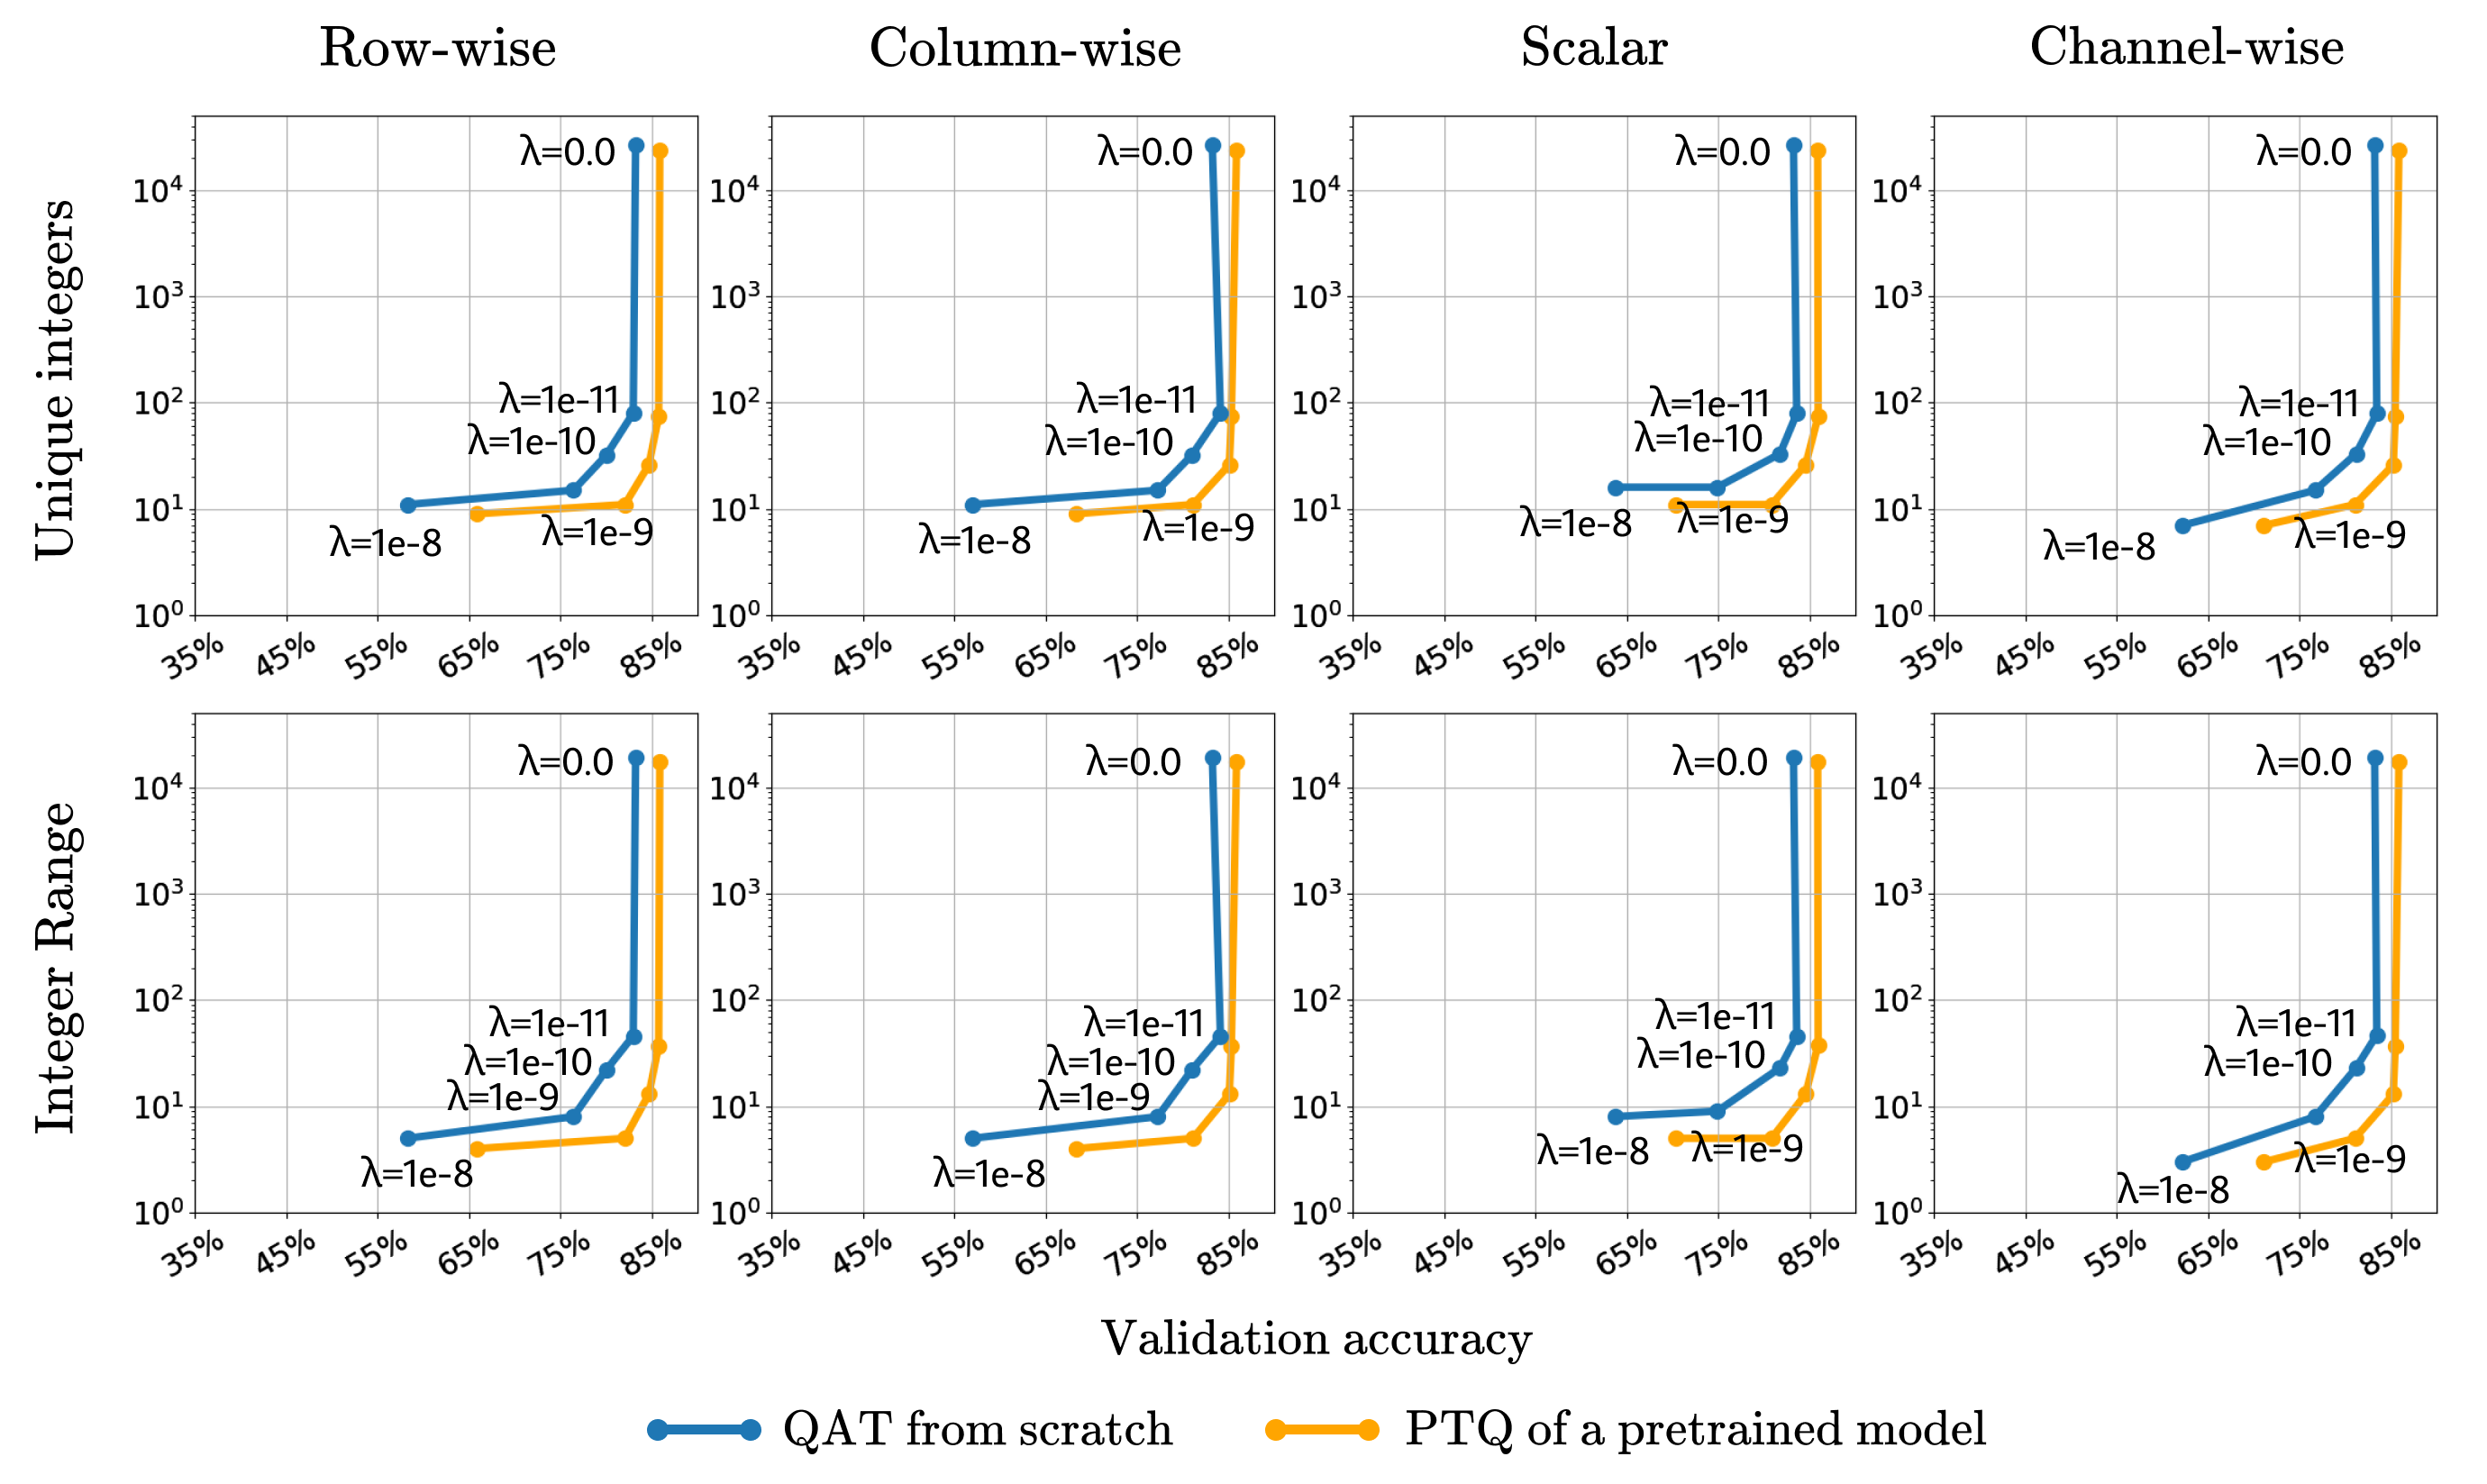
\includegraphics[width=14cm]{Imagenette_nested.png}
  \caption{Accuracy–quantization trade-off for nested quantization layers on Imagenette.}
  \label{fig:imagenette-nested}
\end{figure}


% ------------------------------------------------------------
% ----------------------- Custom loss terms analysis ----------------------- 
% ------------------------------------------------------------
\newpage

\section{Analysis of Custom Loss Terms}
\label{sec:analysisofcustomlossfunctionterms}

\hspace*{1em}For the custom loss term methods, we examine their behavior under different
penalty rates \( \gamma \) for the same three models discussed earlier, 
following a similar approach to the previous section.

% ----------------------- Dense ----------------------- 


\subsection{Fully Connected Layers}
\label{subsec:fullyconnectedlayerscustomloss}

\begin{figure}[t!]
  \centering
  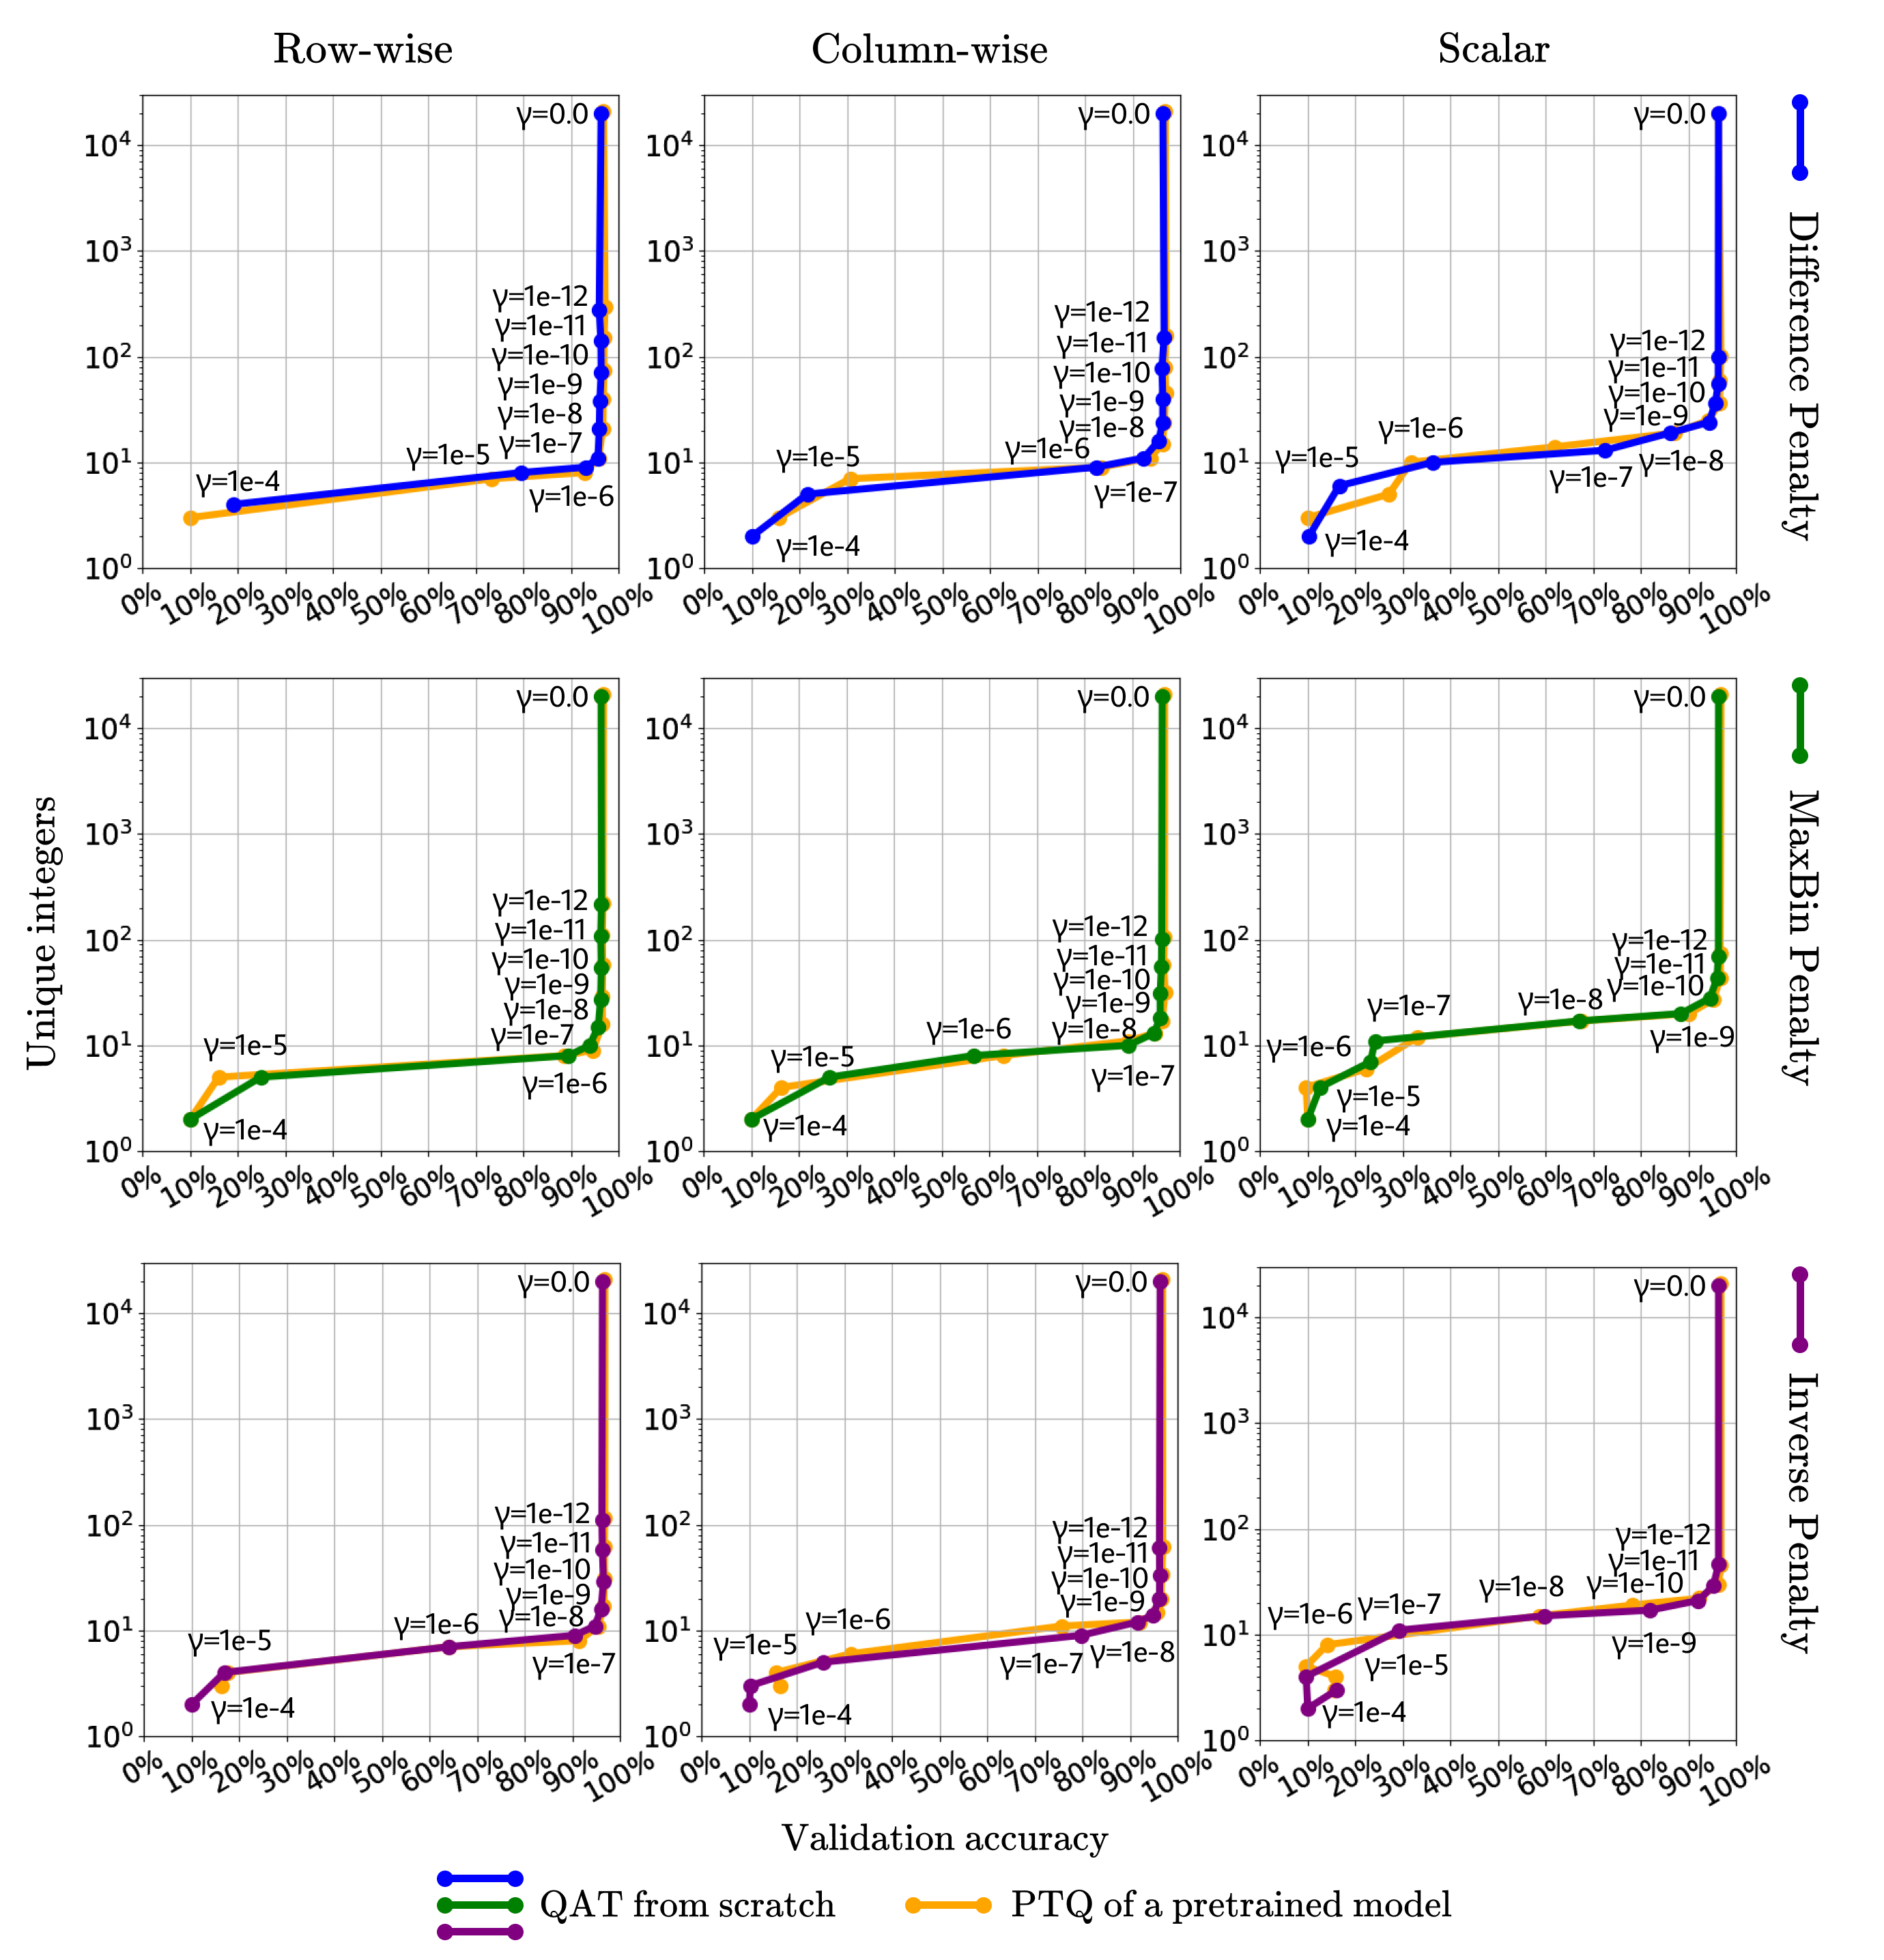
\includegraphics[width=14cm]{mnist_loss.png}
  \caption{Accuracy–quantization trade-off for custom loss terms on MNIST.}
  \label{fig:mnist-loss}
\end{figure}

\hspace*{1em}We compare the three custom loss function terms applied 
to the two dense layers of the model trained on MNIST. 
The resulting Pareto front plots are shown in \cref{fig:mnist-loss}.
We can conclude that the row-wise scenario with the Difference Penalty is the optimal one
as its Pareto front forms the sharpest angle,
the vertex of which is closest to the lower right corner of the plot, indicating an optimal
balance between the number of unique integers and validation accuracy. 
This vertex corresponds to \( \gamma = 1e-7\), that results in integers  
from \(-6 \) to \(2 \),
requiring only \( 4 \) bits, as demonstrated in \cref{fig:quantization_results_1e-7_dense_loss}.

\begin{figure}[t!]
  \centering
  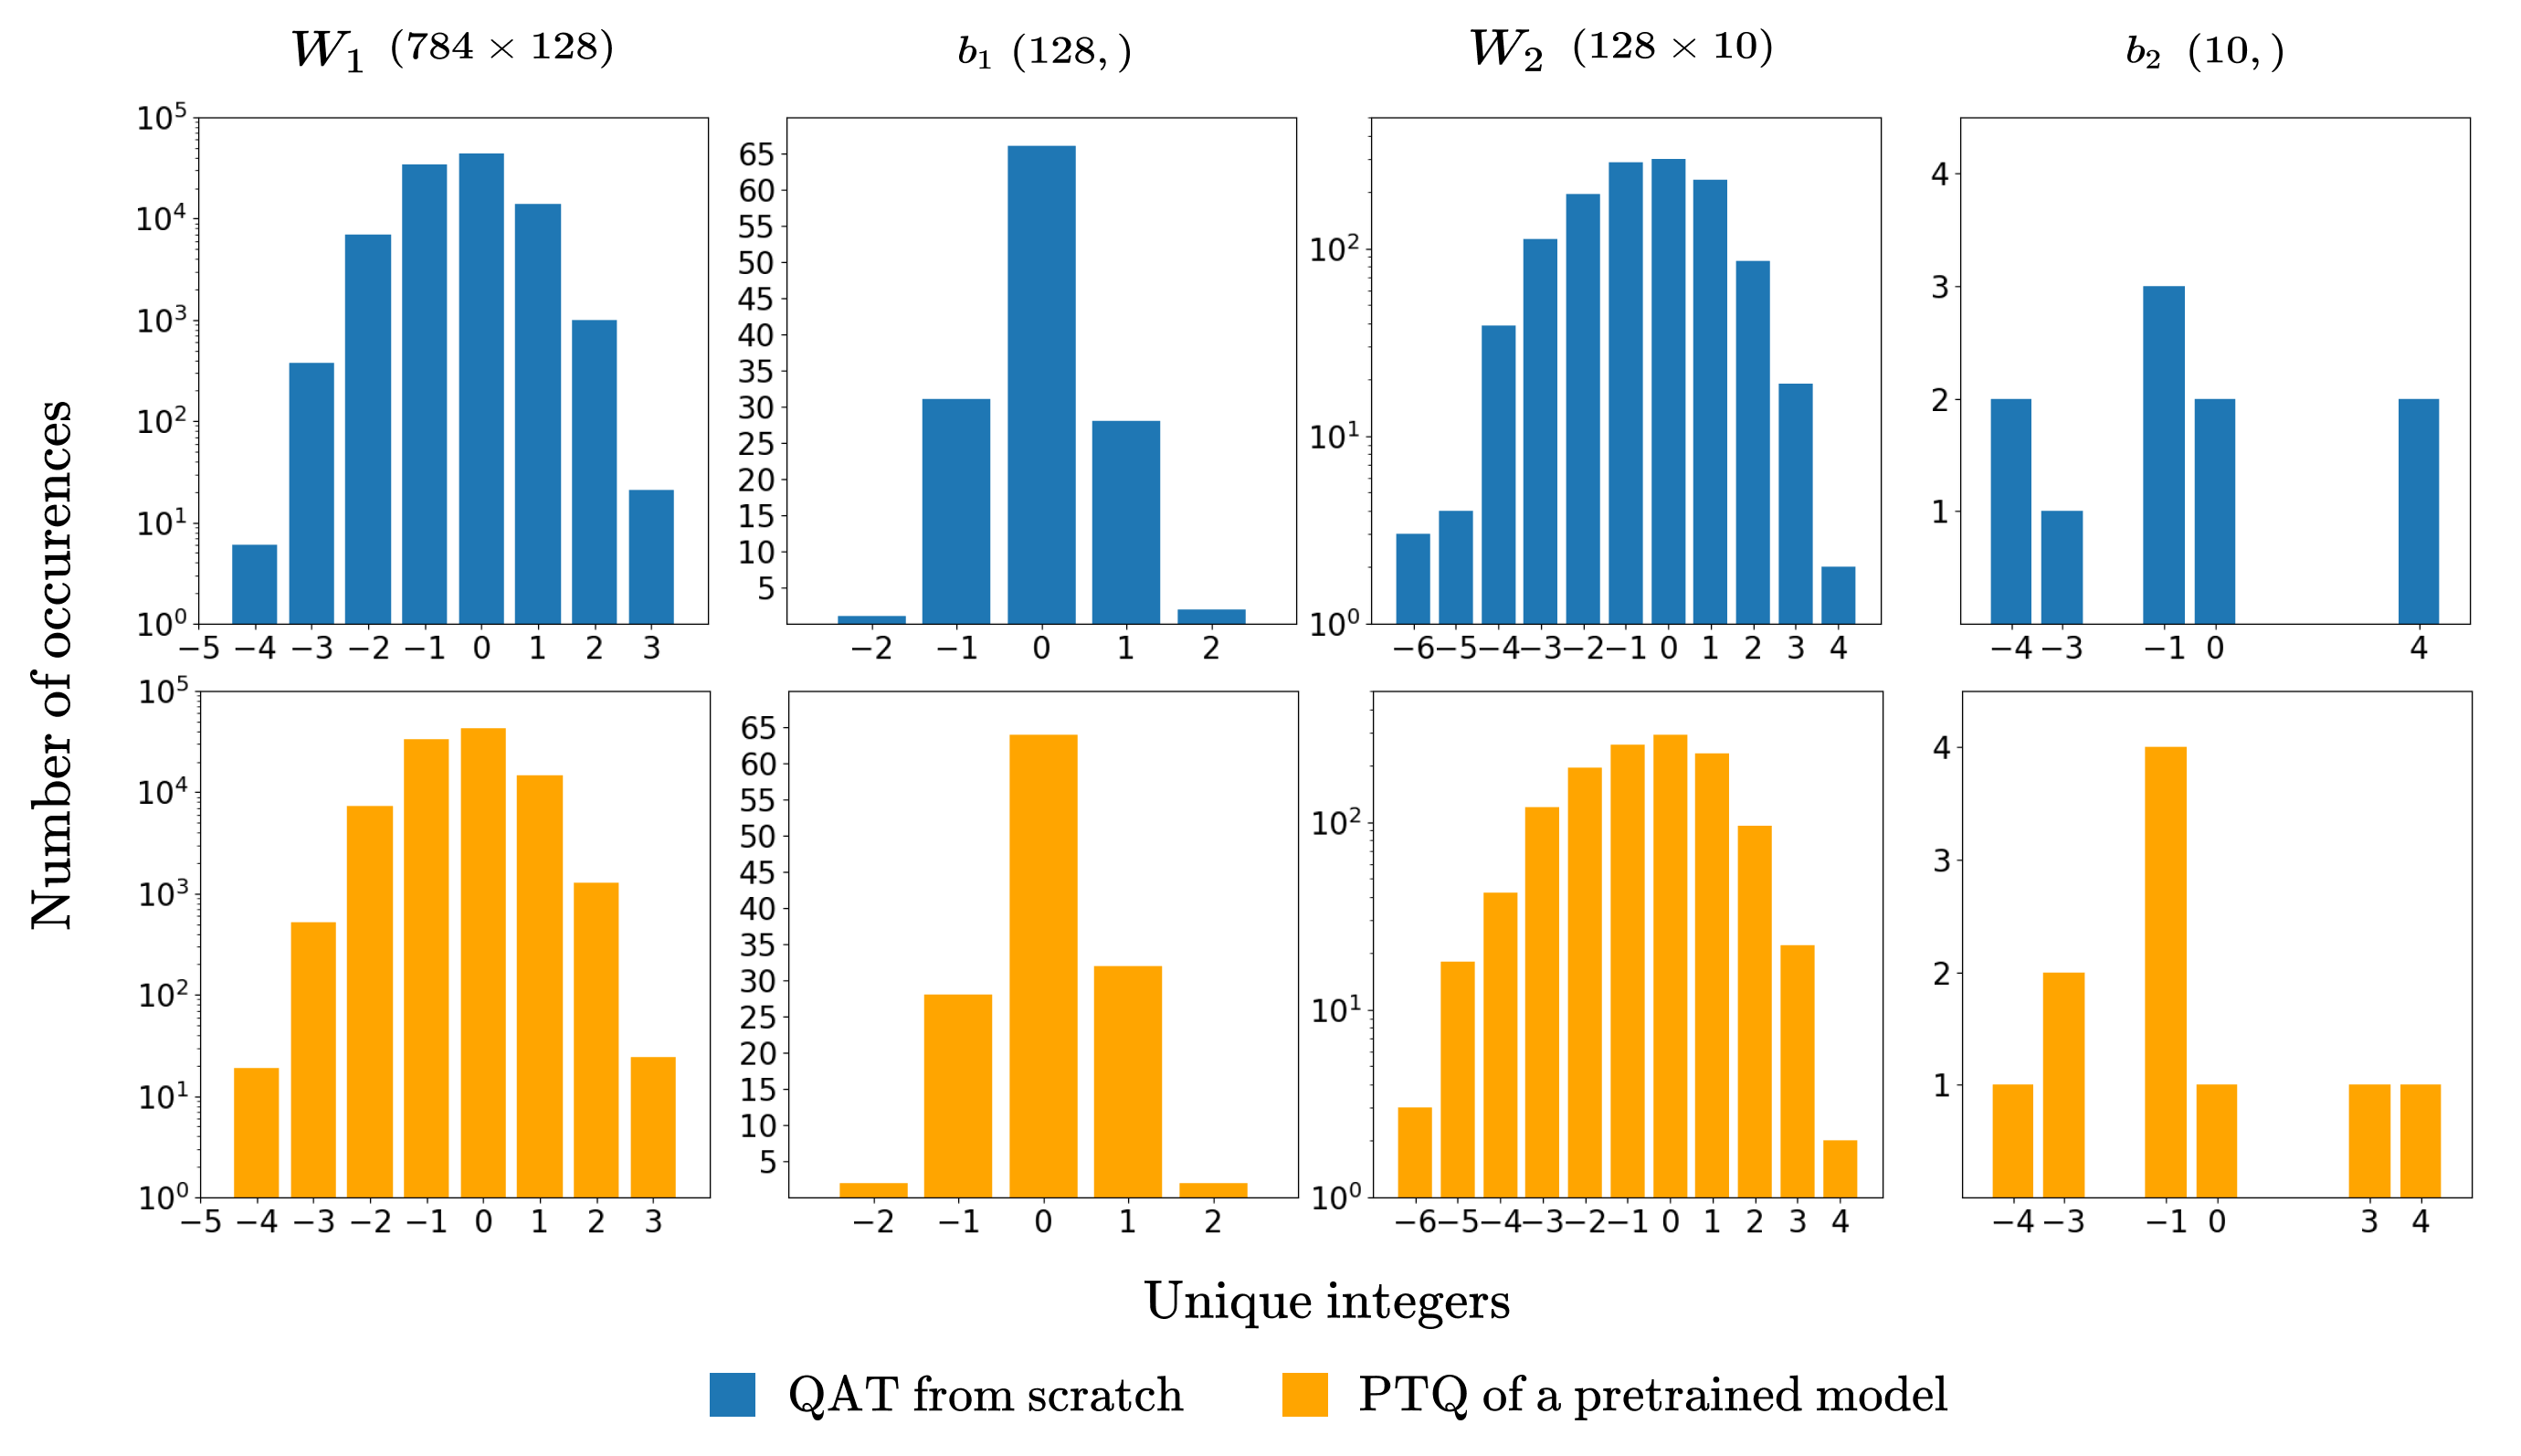
\includegraphics[width=14cm]{quantization_results_1e-7_dense_loss.png}
  \caption{Quantization of MNIST dense layers with row-wise granularity at \( \gamma  = 1e-7 \) with Difference Penalty.}
  \label{fig:quantization_results_1e-7_dense_loss}
\end{figure}

\begin{figure}[t!]
  \centering
  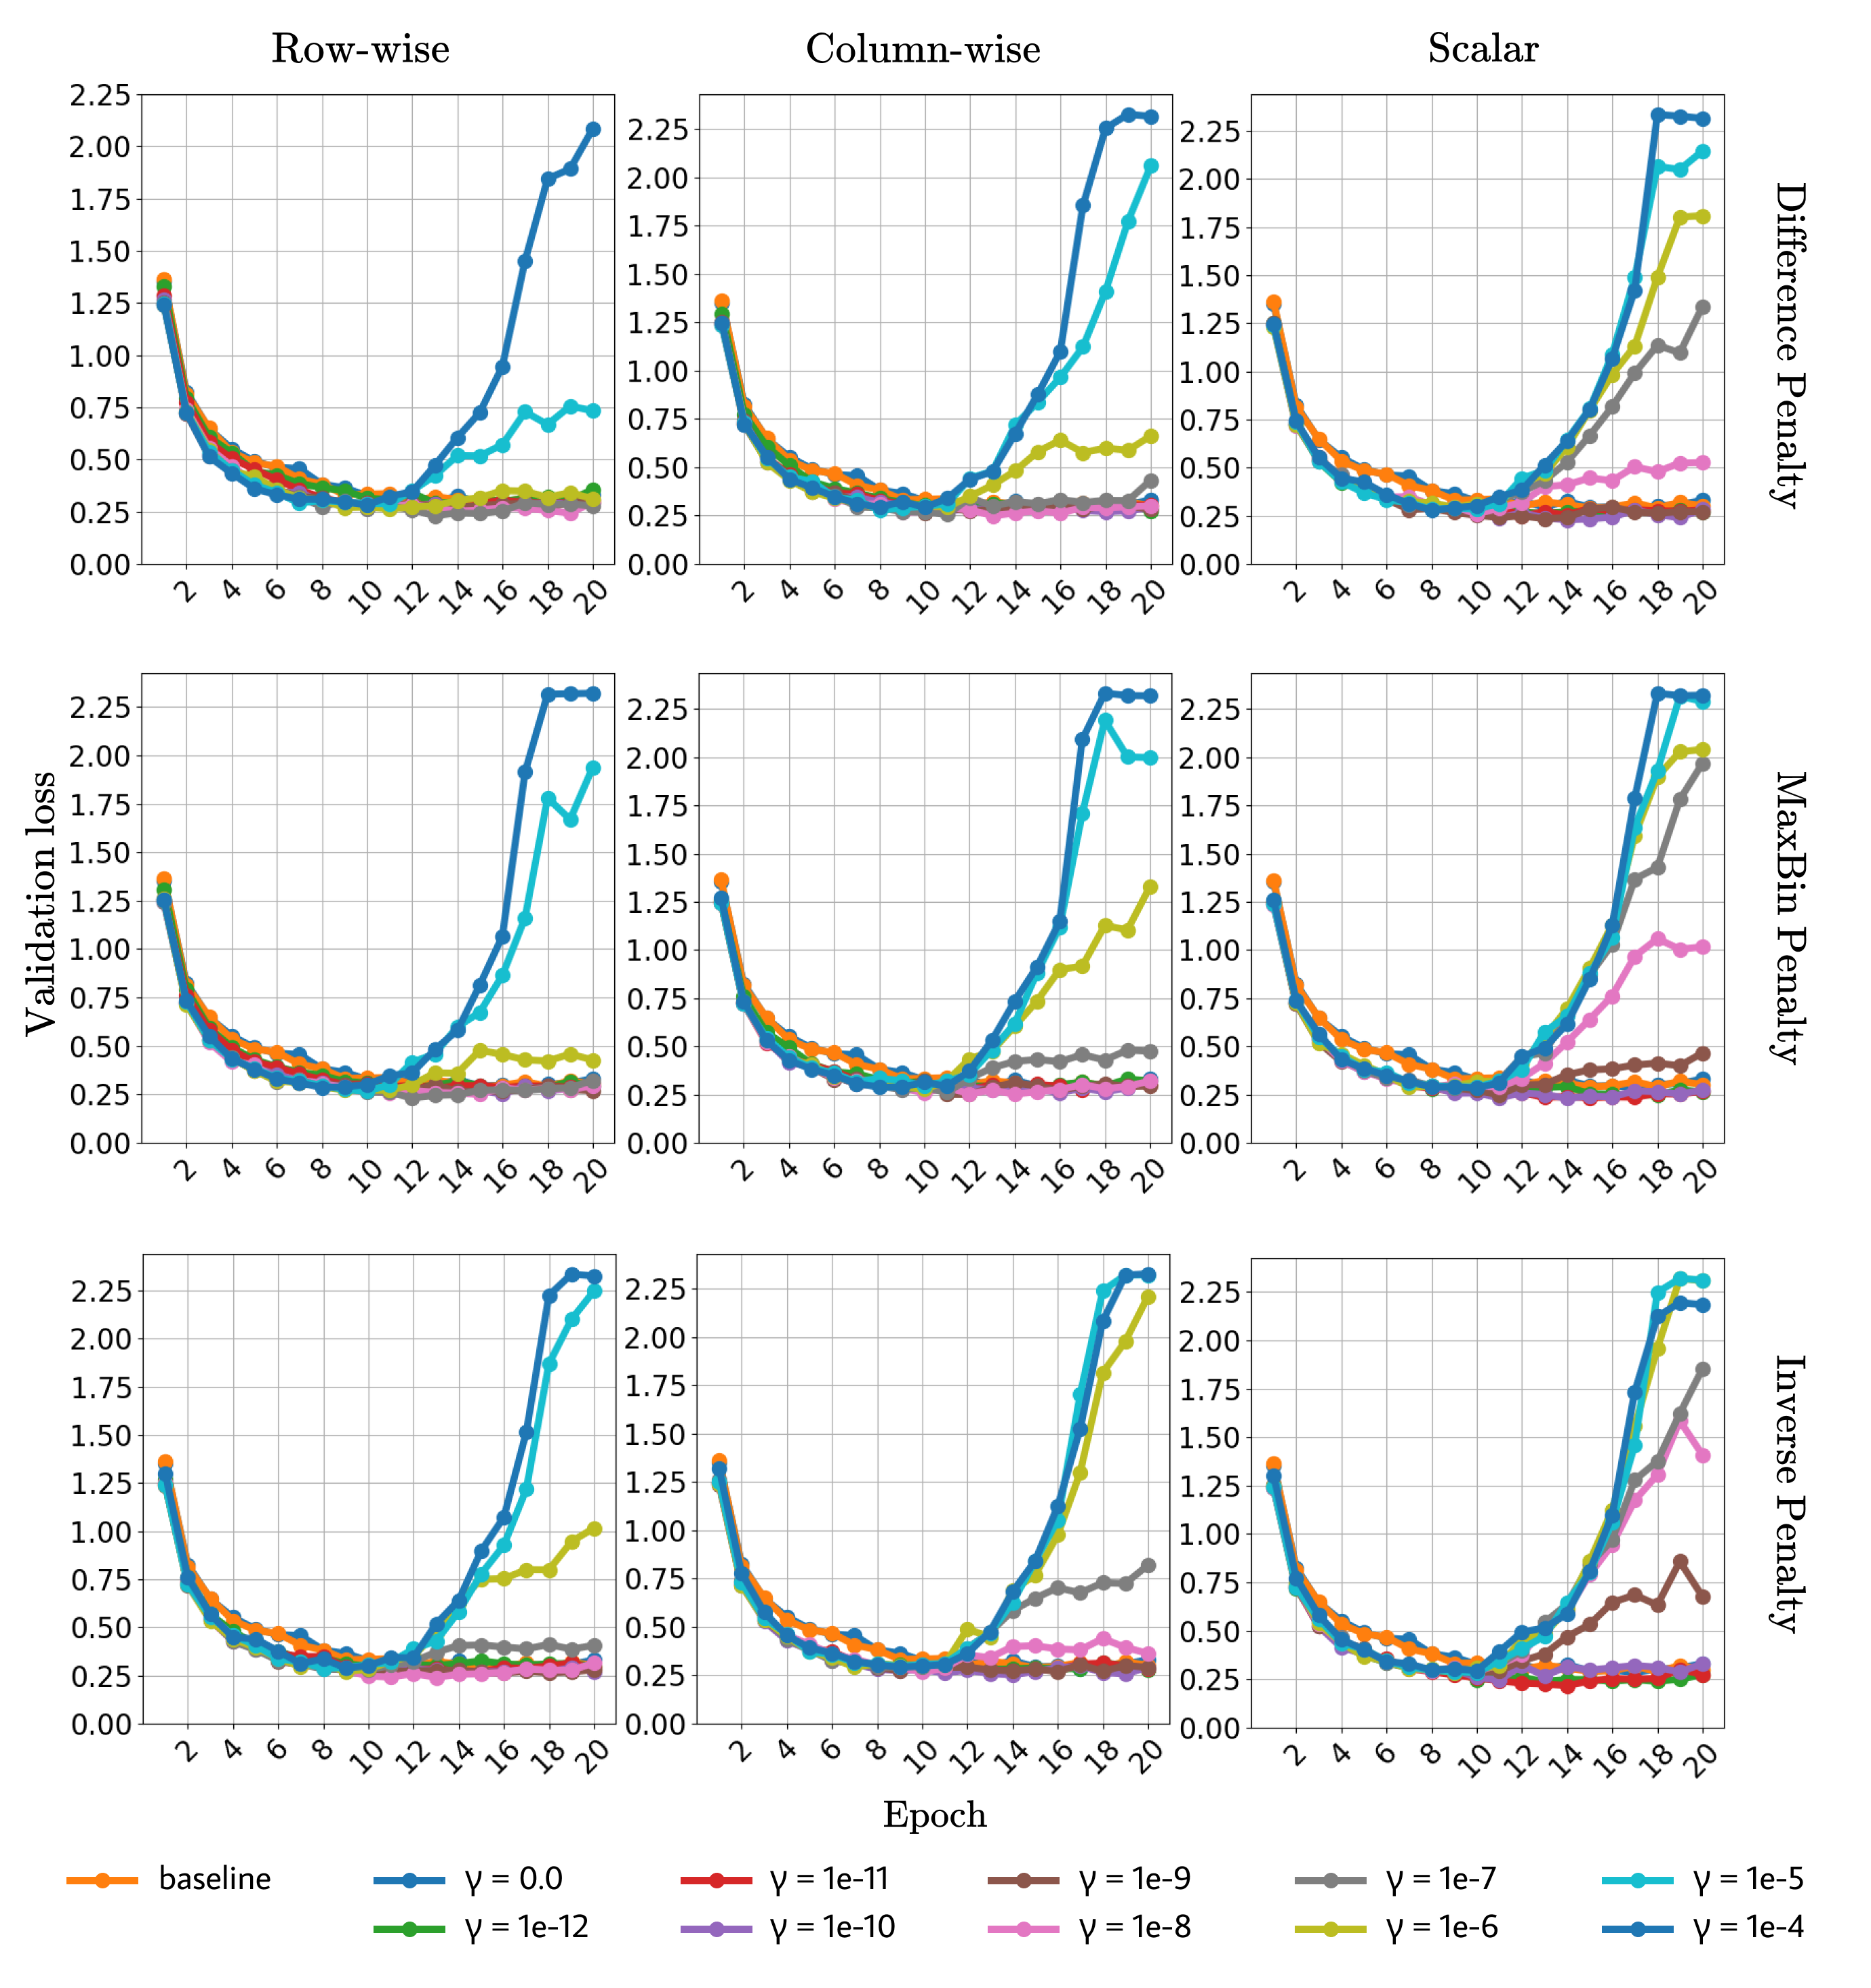
\includegraphics[width=14cm]{mnist-loss-validation.png}
  \caption{Impact of quantization on accuracy and loss for different \( \gamma \) on MNIST.}
  \label{fig:mnist-loss-validation}
\end{figure}

The optimality of the row-wise Difference Penalty case is further supported 
by \cref{fig:mnist-loss-validation}, 
where the validation loss for this scenario starts increasing only at
\( \gamma = 1e-6\), 
while the other granularity and custom loss term combinations
experience a significantly greater increase in loss at the same value of
\( \gamma \). 

From \cref{fig:mnist-loss-validation}, we can make the following additional observations.
First, scalar granularity is the most aggressive among the three granularities, 
resulting in the poorest performance due to its excessive coarseness.
Second, the Inverse Penalty stands out as the most aggressive custom loss term,
which is intuitive, as the scale factors are initialized with very small values, 
leading to larger gradient updates proportional to the inverse of these factors.
Consequently, the combination of scalar granularity and the Inverse Penalty performs the worst among all combinations,
although it still achieves reasonably good quantization,
with fewer than 100 unique integers for  \( \gamma = 1e-12 \).


In terms of PTQ, we observe results approximately similar to those of QAT from scratch, 
as shown in \cref{fig:mnist-loss} and \cref{fig:quantization_results_1e-7_dense_loss}. 
The progression of validation loss for each scenario follows the same pattern as in \cref{fig:mnist-loss-validation}, 
although the initial value at the start of training is closer to 0.25 due to the use of a pretrained model.


\newpage

% ----------------------- Conv ----------------------- 

\subsection{Convolutional Layers}
\label{subsec:convolutionallayerscustomloss}

\hspace*{1em} We now compare the loss function terms applied to the convolutional layers of the model trained on CIFAR-10. 
Based on the results summarized in \cref{fig:cifar-loss} and \cref{fig:cifar-loss-validation}, 
the conclusion that the scalar granularity combined with the Inverse Penalty approach is the most aggressive remains valid. 
However, we observe that the channel-wise granularity is the most suitable configuration in this case, 
with \( \gamma = 1e-10 \) producing integers ranging from -28 to 34 in the kernels of the convolutional layers.
These integers form a bell curve closely resembling the experimental results of the nested quantization layer
with row-wise granularity for \( \lambda = 1e-11\) depicted in \cref{fig:quantization-results-1e-10conv}
\begin{figure}[t!]
  \centering
  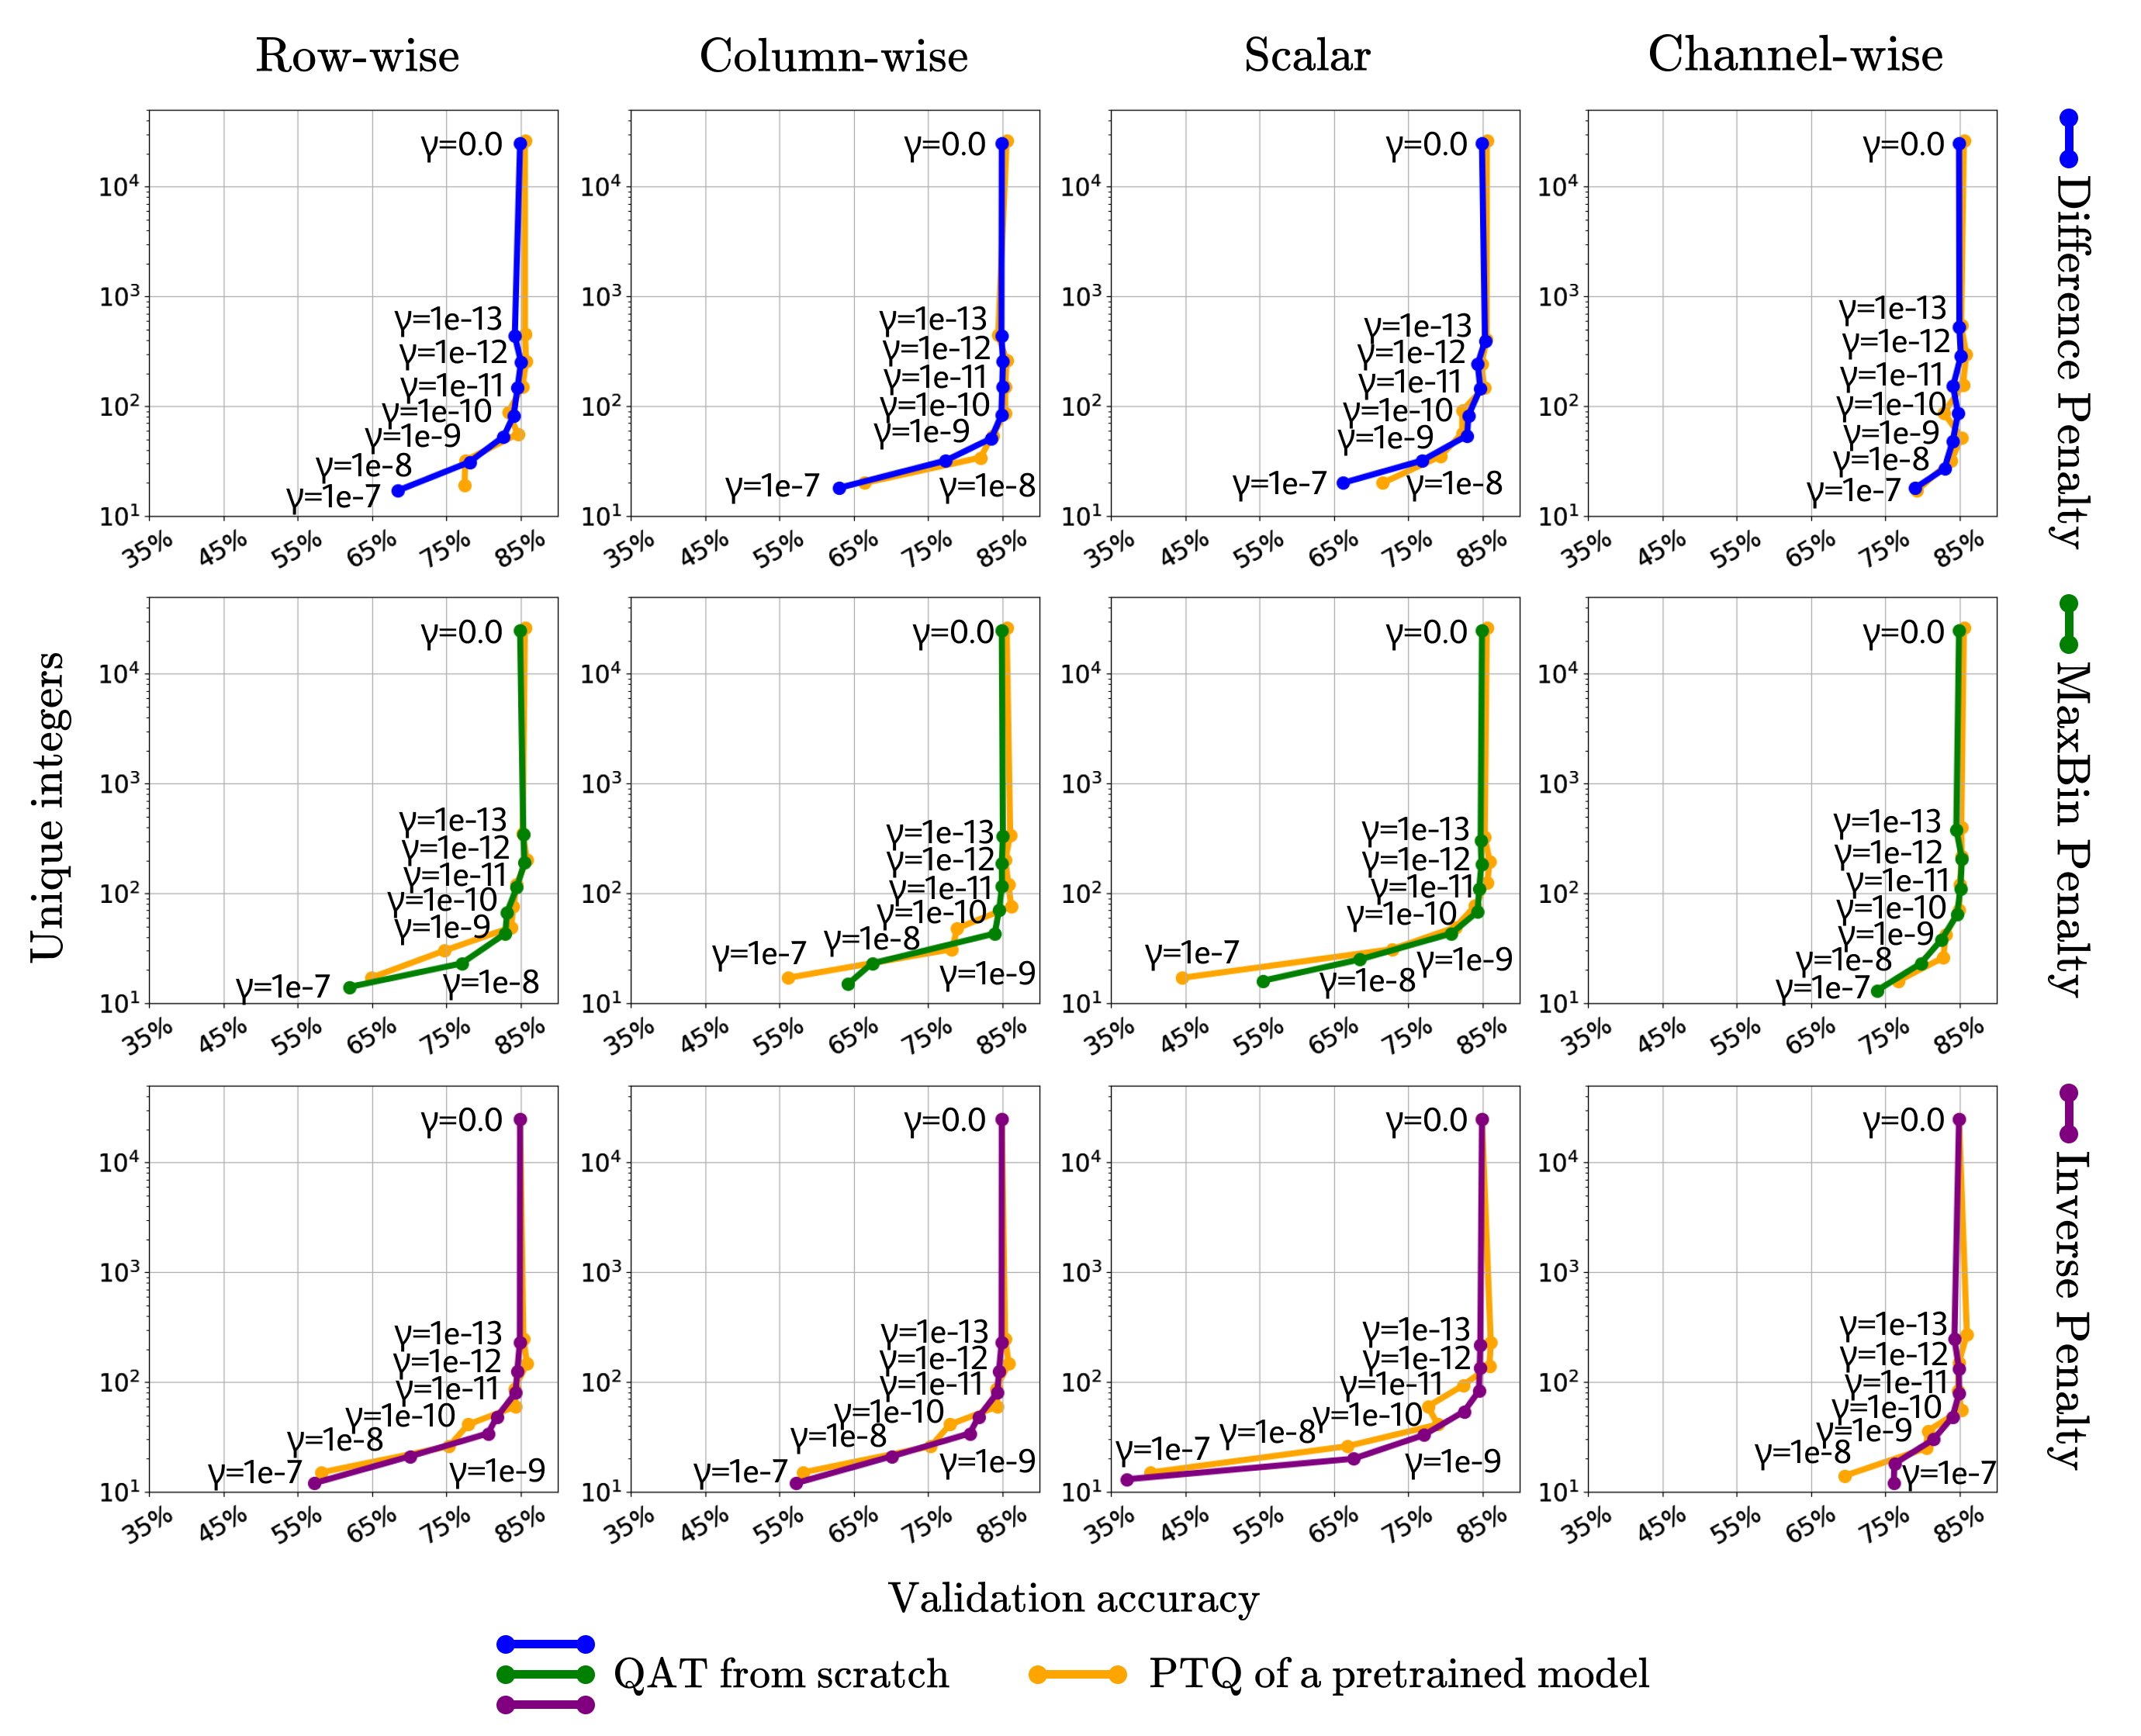
\includegraphics[width=14cm]{cifar_loss.png}
  \caption{Accuracy–quantization trade-off for custom Loss terms on CIFAR-10.}
  \label{fig:cifar-loss}
\end{figure}
It is worth noting that, 
compared to the gradient-based nested quantization layer approach, the custom loss terms
lead to more outliers in the resulting integers of biases.
This behavior can be attributed to the custom loss term formulations, 
specifically how they are scaled with the number of parameters in each kernel and bias.
Since the bias scale factors affect significantly fewer individual parameters than the kernels, 
their contribution to the loss term is smaller, leading to much smaller updates.

\begin{figure}[t!]
  \centering
  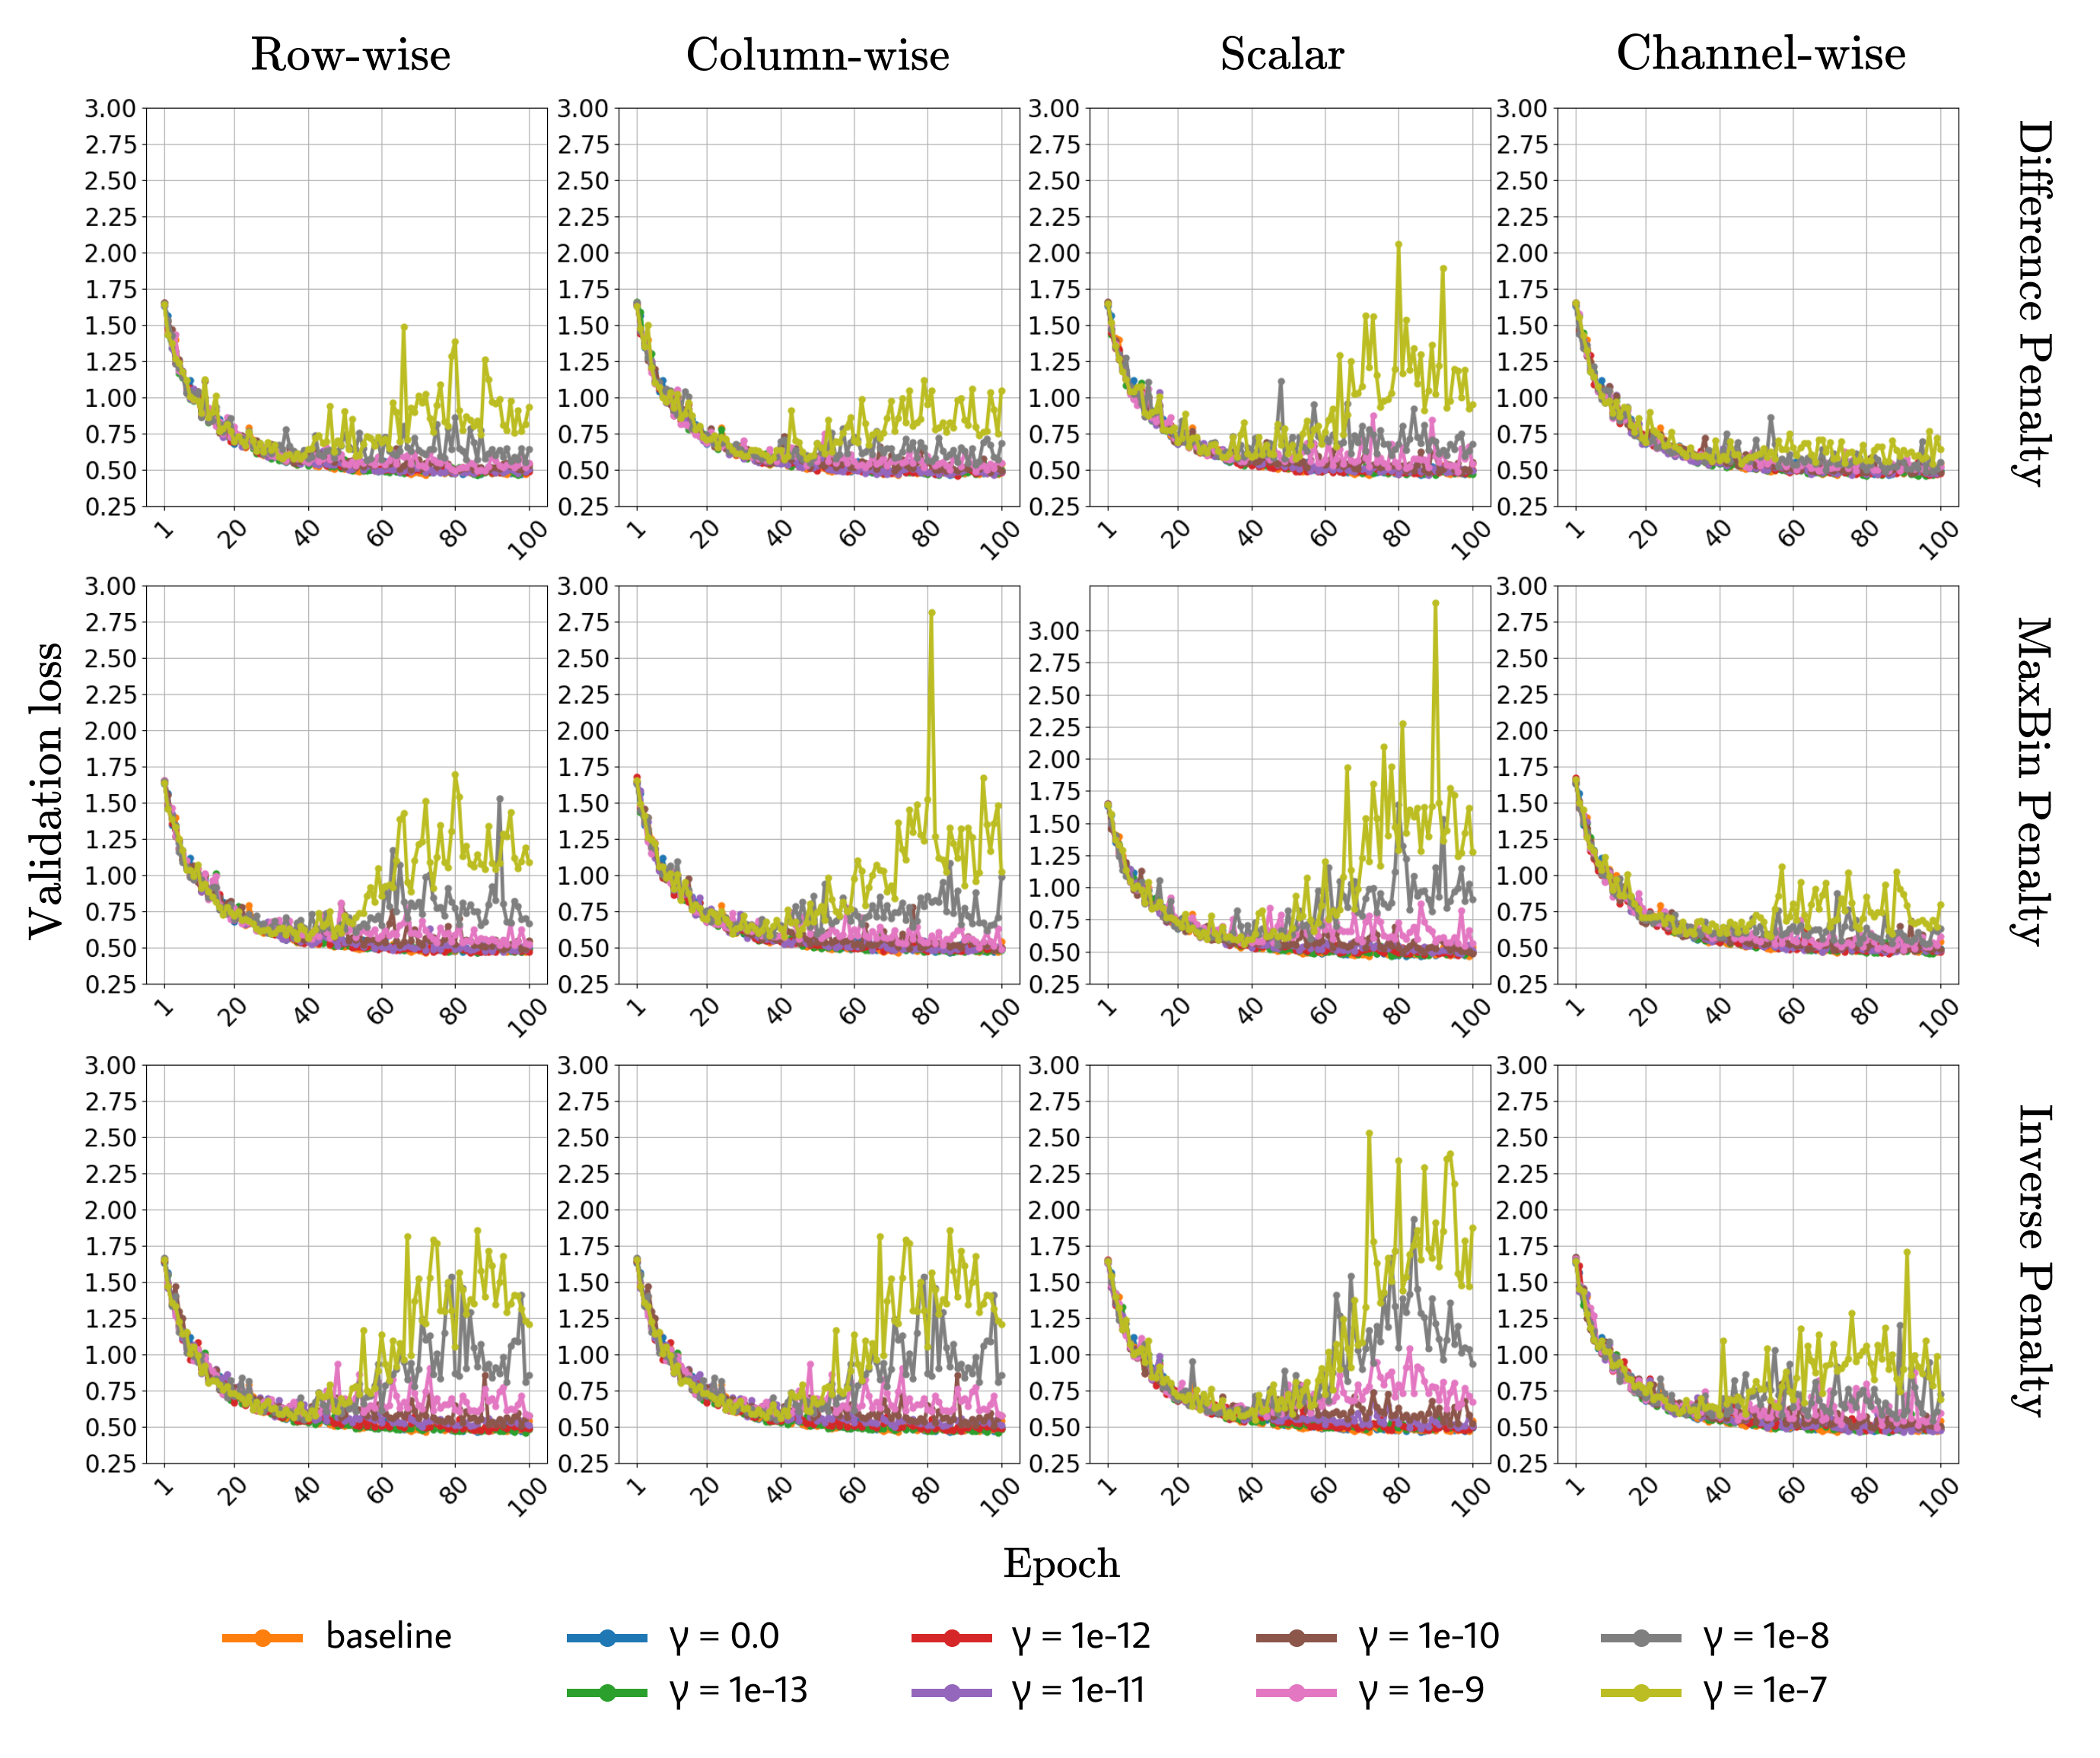
\includegraphics[width=14cm]{cifar-loss-validation.png}
  \caption{Impact of quantization on accuracy and for different \( \gamma \) and custom loss function terms on CIFAR-10.}
  \label{fig:cifar-loss-validation}
\end{figure}

Similar to the other experiments, we conduct PTQ using a full-precision pretrained model. 
The results of PTQ are closely comparable to those obtained through QAT as evident from \cref{fig:cifar-loss}
— which demonstrates the effectiveness of learned quantization in achieving similar outcomes 
without the need for a separate pretraining phase.
Furthermore, the PTQ results for the channel-wise granularity and Difference Penalty combination we highlighted earlier
align closely with those observed in the learned quantization scenario.

\begin{figure}[t!]
  \centering
  \includegraphics[width=14cm]{imagenette_loss.png}
  \caption{Accuracy–quantization trade-off for custom loss terms on Imagenette.}
  \label{fig:imagenette-loss}
\end{figure}

For the model trained on Imagenette, 
the custom loss terms fail to form a Pareto front as depicted in \cref{fig:imagenette-loss}, 
although reasonable quantization is achieved with minimal accuracy loss. 
This behavior is attributed to the learning rate decay, 
which prevents the model from reaching a quantization level that could significantly 
impact accuracy once the learning rate becomes too small. In contrast, 
the nested quantization layer approach quantizes more rapidly, ultimately 
"breaking" the model for larger values of the corresponding 
hyperparameter before the learning rate decay limits further updates.

Nevertheless, for the Imagenette dataset, we observe improved accuracy in the PTQ scenario
as noticed in the case with the nested quantization layer. 

Table~\ref{tab:losscomrpessionrate} presents the file sizes of dense or convolutional layers before and after applying our PTQ in selected training scenarios. 
For demonstration purposes, we use the same compression technique as in the nested quantization layer approach.
Across all datasets, we observe a substantial reduction in file size, with reductions sometimes exceeding a factor of 10. 

\begin{table}[t!]
  \centering
  \caption{Compression rate for chosen quantization scenarios}
  \label{tab:losscomrpessionrate}
  \begin{tabular}{lccc}
      \toprule
      \textbf{Combination}     & \textbf{Baseline} & \textbf{PTQ + Compression} & \textbf{Granularity, $\gamma$} \\ 
      \midrule
      MNIST, Difference               & $\approx 0.36 $ MB            & $\approx 0.03 $ MB              & row-wise, $1e-7$         \\ 
      MNIST, MaxBin               & $\approx 0.36 $ MB             & $\approx 0.04 $ MB             &  row-wise, $ 1e-8$           \\ 
      MNIST, Inverse               & $\approx 0.36 $ MB            & $\approx 0.04 $ MB             &  row-wise, $1e-9$          \\ 
      CIFAR-10, Difference          &  $\approx 1.02 $ MB          & $\approx 0.17 $ MB            & channel-wise, $1e-10$            \\ 
      CIFAR-10, MaxBin               &  $\approx 1.02 $ MB            & $\approx 0.15 $ MB              &channel-wise, $ 1e-10$          \\ 
      CIFAR-10, Inverse               &  $\approx 1.02 $ MB            &$\approx 0.16 $ MB              &channel-wise, $1e-11$           \\ 
      Imagenette, Difference               &  $\approx 39.57 $ MB            & $\approx 5.90 $ MB              &channel-wise, $ 1e-9$            \\ 
      Imagenette, MaxBin               &  $\approx 39.57 $ MB        & $\approx 6.46 $ MB             & channel-wise, $1e-9$            \\ 
      Imagenette, Inverse               &  $\approx 39.57 $ MB          & $\approx 5.37 $ MB             & channel-wise, $1e-8$          \\ 

      \bottomrule
  \end{tabular}
  \vspace{1.0em}
\end{table}